%\mbox{}\newpage
\chapter{\hspace{-1mm}\bf 数值实验}
\label{chap6}
\addcontentsline{toe}{chapter}{{{\bf Chapter \currentchapter \ 
Numerical Experiments }}\numberline\,}
\markboth{第 \currentchapter \ 章
数值实验}{北京航空航天大学博士后研究工作报告}

%%%%%%%%%%%%%%%%%%%%%%%%%%%%%%%%%%%%%%%%%%%%%%%%%%%%%%%%%%%

本章对本文前面几个章节介绍的部分联邦学习算法进行数值上的评测。评测主要从算法的整体效果 (在测试集上的准确度、损失,以及收敛速度等);对于子节点参与联邦训练比例的鲁棒性;以及对学习率等超参数的敏感性等几个方面进行。为了排除随机因素的干扰,每一组实验都使用了5个不同的随机数种子 (一般都被设为$0, 1, 2, 3, 4$) 进行重复试验,最后得到结果的形式的是均值曲线$\pm$误差界,误差界在这里选取的是标准差。

由于本文成文时间的关系,本章的数值试验大部分使用的是上一章\S\ref{sec:chap5-datasets}中介绍的小规模的联邦数据集\texttt{FedProxFEMNIST}。选择这个数据集是基于如下的原因:
\begin{itemize}
    \item \texttt{FedProxFEMNIST}数据集来源自真实数据集EMNIST\cite{cohen2017emnist},后者被广泛采用为测试机器学习模型的基准数据集。
    \item \texttt{FedProxFEMNIST}数据集的数据分割方式使得子节点之间的数据是非独立同分布的,而且天然形成了10个聚落的结构,方便评测聚类联邦学习算法\cite{Ghosh_2022_cfl, Sattler_2021_cfl}在内的多种联邦学习算法的鲁棒性。
    \item \texttt{FedProxFEMNIST}数据集的数据规模较小,非常适合联邦学习算法的快速验证工作。
\end{itemize}

\section{联邦学习算法整体效果的数值评测}
\addcontentsline{toe}{section}{{\currentchapter .1\ \ Numerical Evaluation of the Overall Effectiveness of Federated Learning Algorithms}\numberline\,}
\label{sec:chap6-overall}

% almost finished

本节对几种典型的联邦学习算法进行数值上的评测,包括
\begin{itemize}
    \item \texttt{FedAvg}\cite{mcmahan2017fed_avg} (作为\texttt{FedOpt}\cite{reddi2020fed_opt}的特例),
    \item \texttt{FedAdam}\cite{reddi2020fed_opt, adam} (作为\texttt{FedOpt}\cite{reddi2020fed_opt}的特例),
    \item \texttt{FedAdagrad}\cite{reddi2020fed_opt, adagrad} (作为\texttt{FedOpt}\cite{reddi2020fed_opt}的特例),
    \item \texttt{FedYogi}\cite{reddi2020fed_opt, Zaheer_2018_yogi} (作为\texttt{FedOpt}\cite{reddi2020fed_opt}的特例),
    \item \texttt{FedProx}\cite{sahu2018fedprox},
    \item \texttt{Ditto}\cite{li_2021_ditto},
    \item \texttt{FedSplit}\cite{pathak2020fedsplit},
    \item \texttt{IFCA}\cite{Ghosh_2022_cfl},
    \item \texttt{ProxSkip}\cite{proxskip}.
\end{itemize}
各个算法的超参数的设置基本与\S\ref{sec:chap5-design}中展示的典型的联邦学习仿真系统\texttt{fl-sim}命令行接口配置文件\ref{lst:fl-sim-config}~一致,即整体进行100轮次的迭代循环;在每一轮循环内,子节点以步长0.03执行10步子问题迭代训练,训练数据的批大小 (Batch Size)\index{批大小, Batch Size} 采用数据集\texttt{FedProxFEMNIST}预置的默认批大小,值为20.

\begin{figure}[ht]
    \centering
    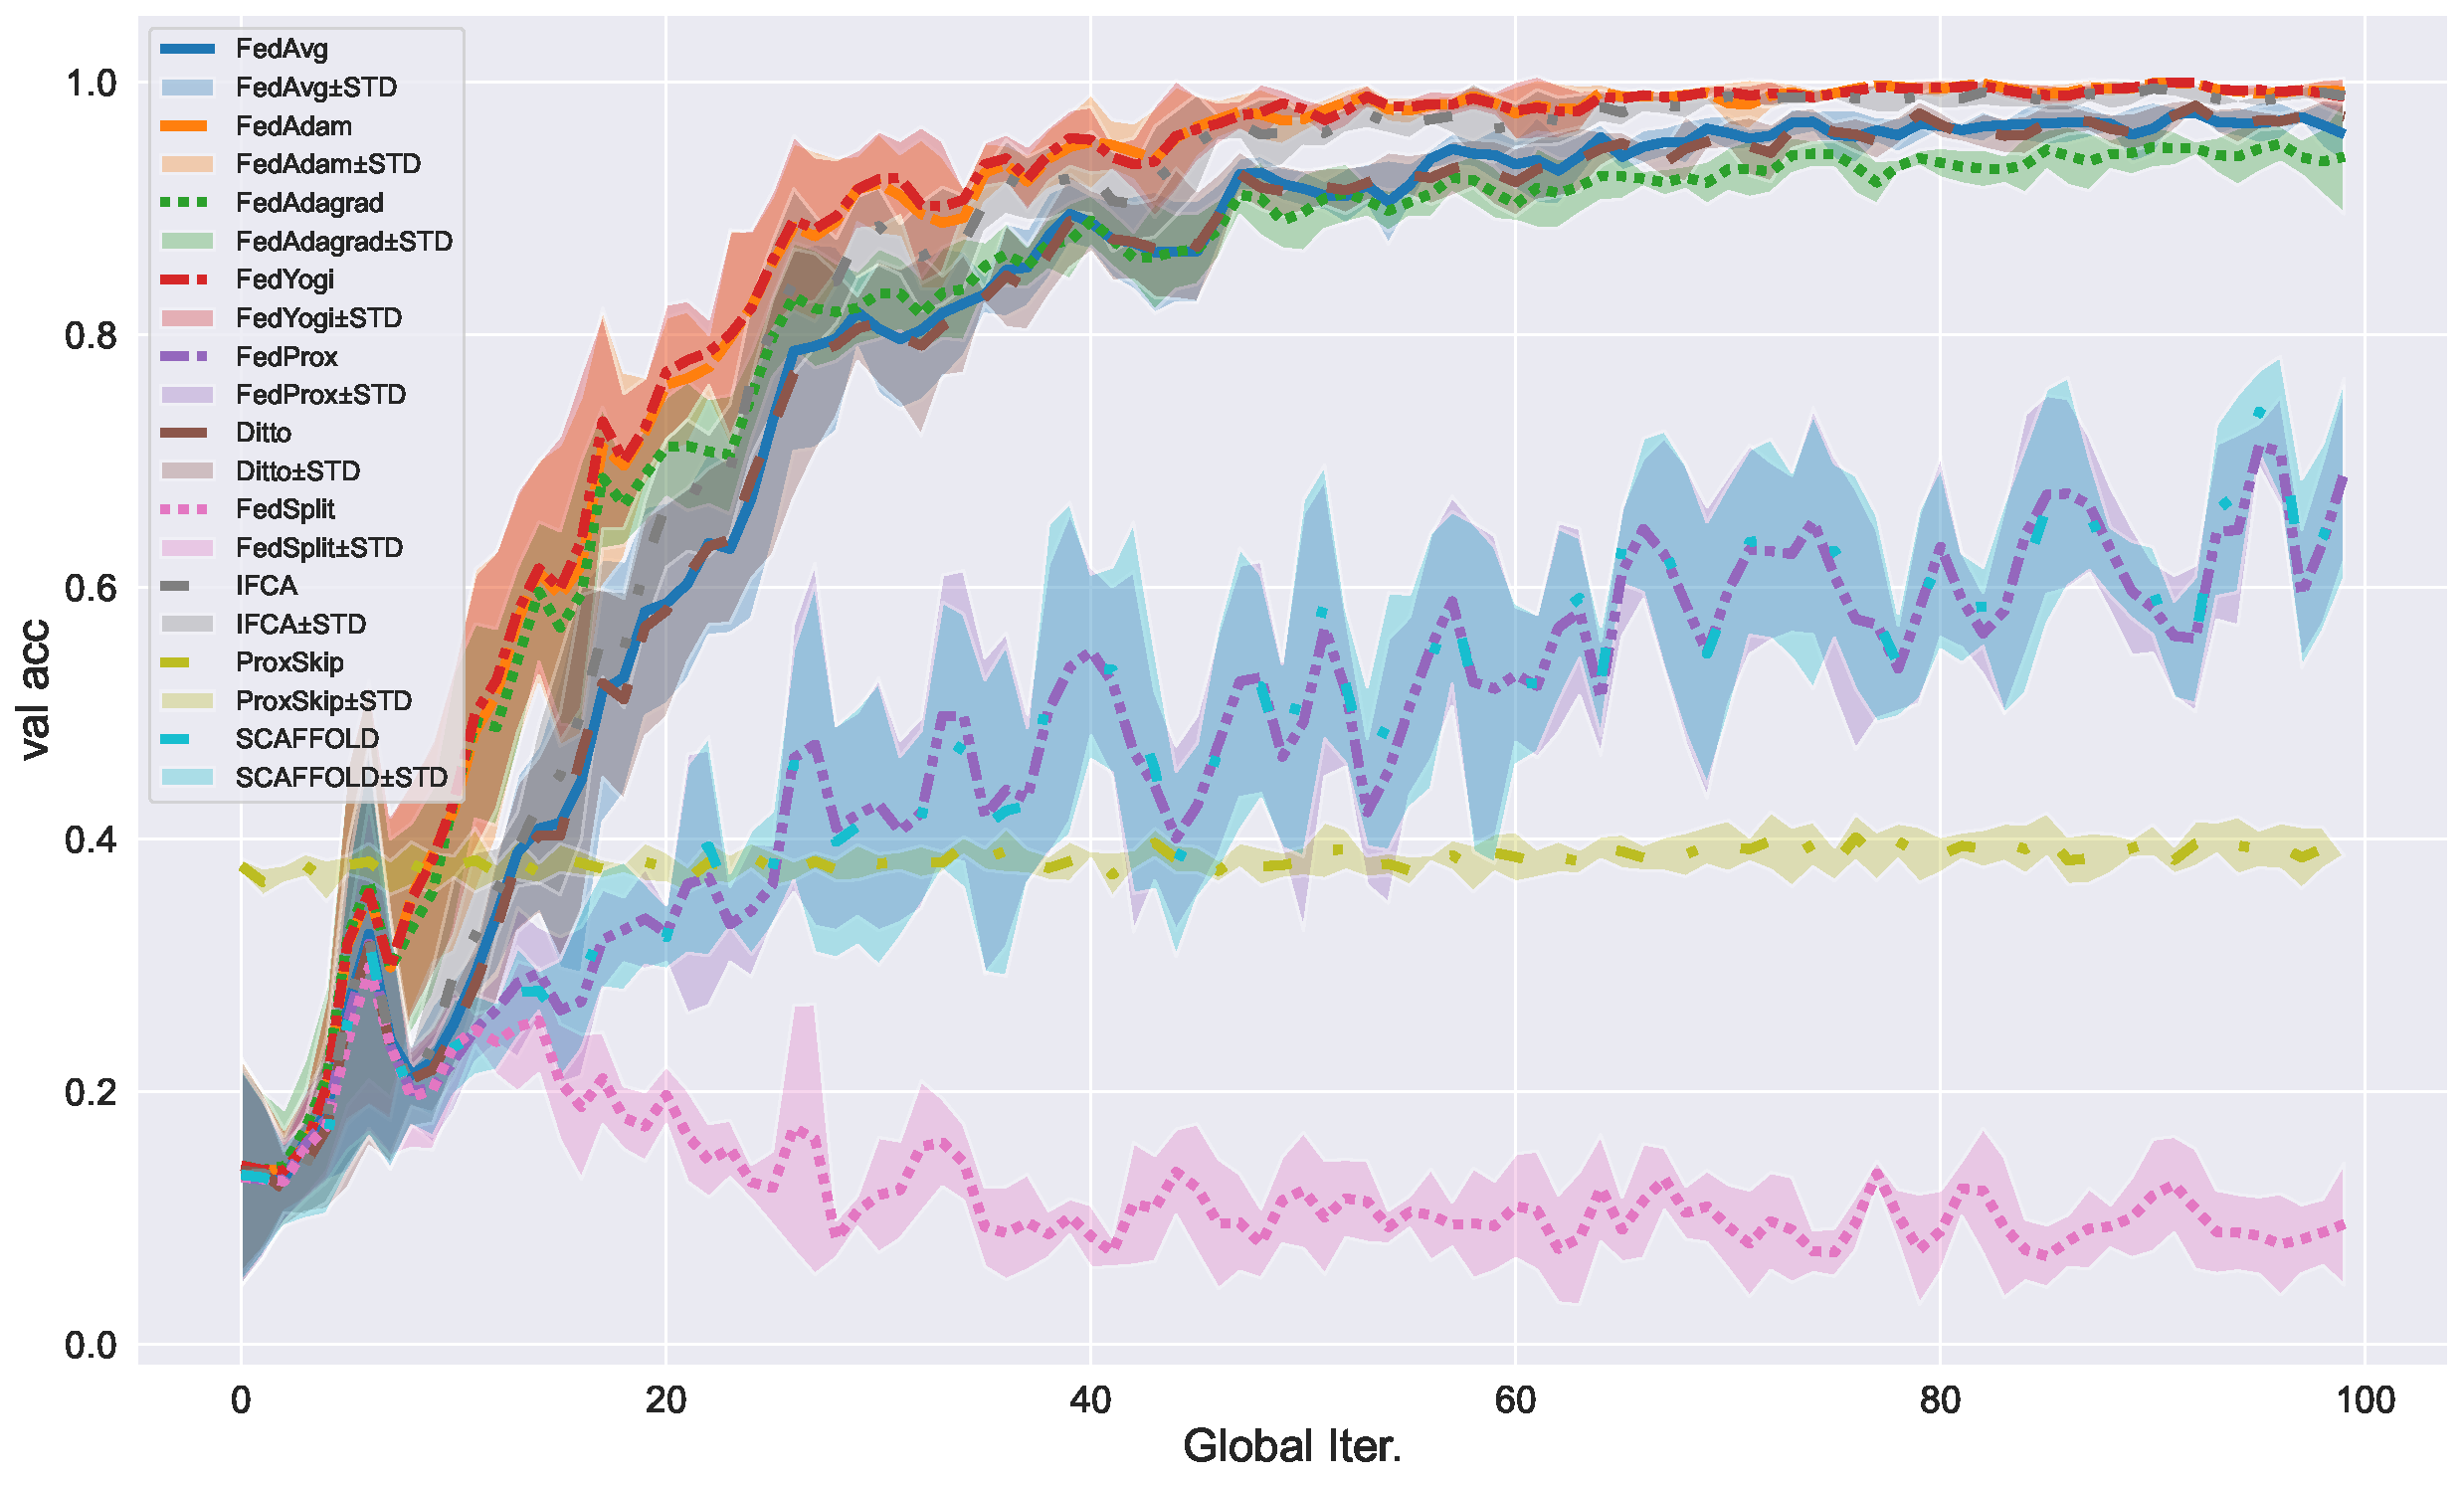
\includegraphics[width=0.9\textwidth]{figures/standard-test-ratio-10-val-acc.pdf}
    \caption{几种典型的联邦学习算法在子节点参与训练比例为$10\%$时,在测试集上的准确率曲线}
    \label{fig:standard-test-ratio-10-val-acc}
\end{figure}

图\ref{fig:standard-test-ratio-10-val-acc}~是以上列出的几种联邦学习优化算法在在子节点参与训练比例为$10\%$ (或者等价地,子节点掉队 (Straggler) 几率为$90\%$) 的场景下,在数据集\texttt{FedProxFEMNIST}的测试集上的准确率曲线。可以看到\texttt{FedOpt}相关的几种算法:\texttt{FedAdam}, \texttt{FedAdagrad}, \texttt{FedYogi}, 包括\texttt{FedAvg},在这种比较极端的场景下,都有非常不错的鲁棒性。除此之外,\texttt{IFCA}, \texttt{Ditto}等算法在这种场景下的鲁棒性也不错。而联邦临近算法\texttt{FedProx}在这种场景下的模型准确率曲线波动比较剧烈,而且在整体100轮的迭代之后还未收敛。\texttt{ProxSkip}以及\texttt{FedSplit}算法在子节点参与训练比例为$10\%$的场景下发散。

\begin{figure}[ht]
    \centering
    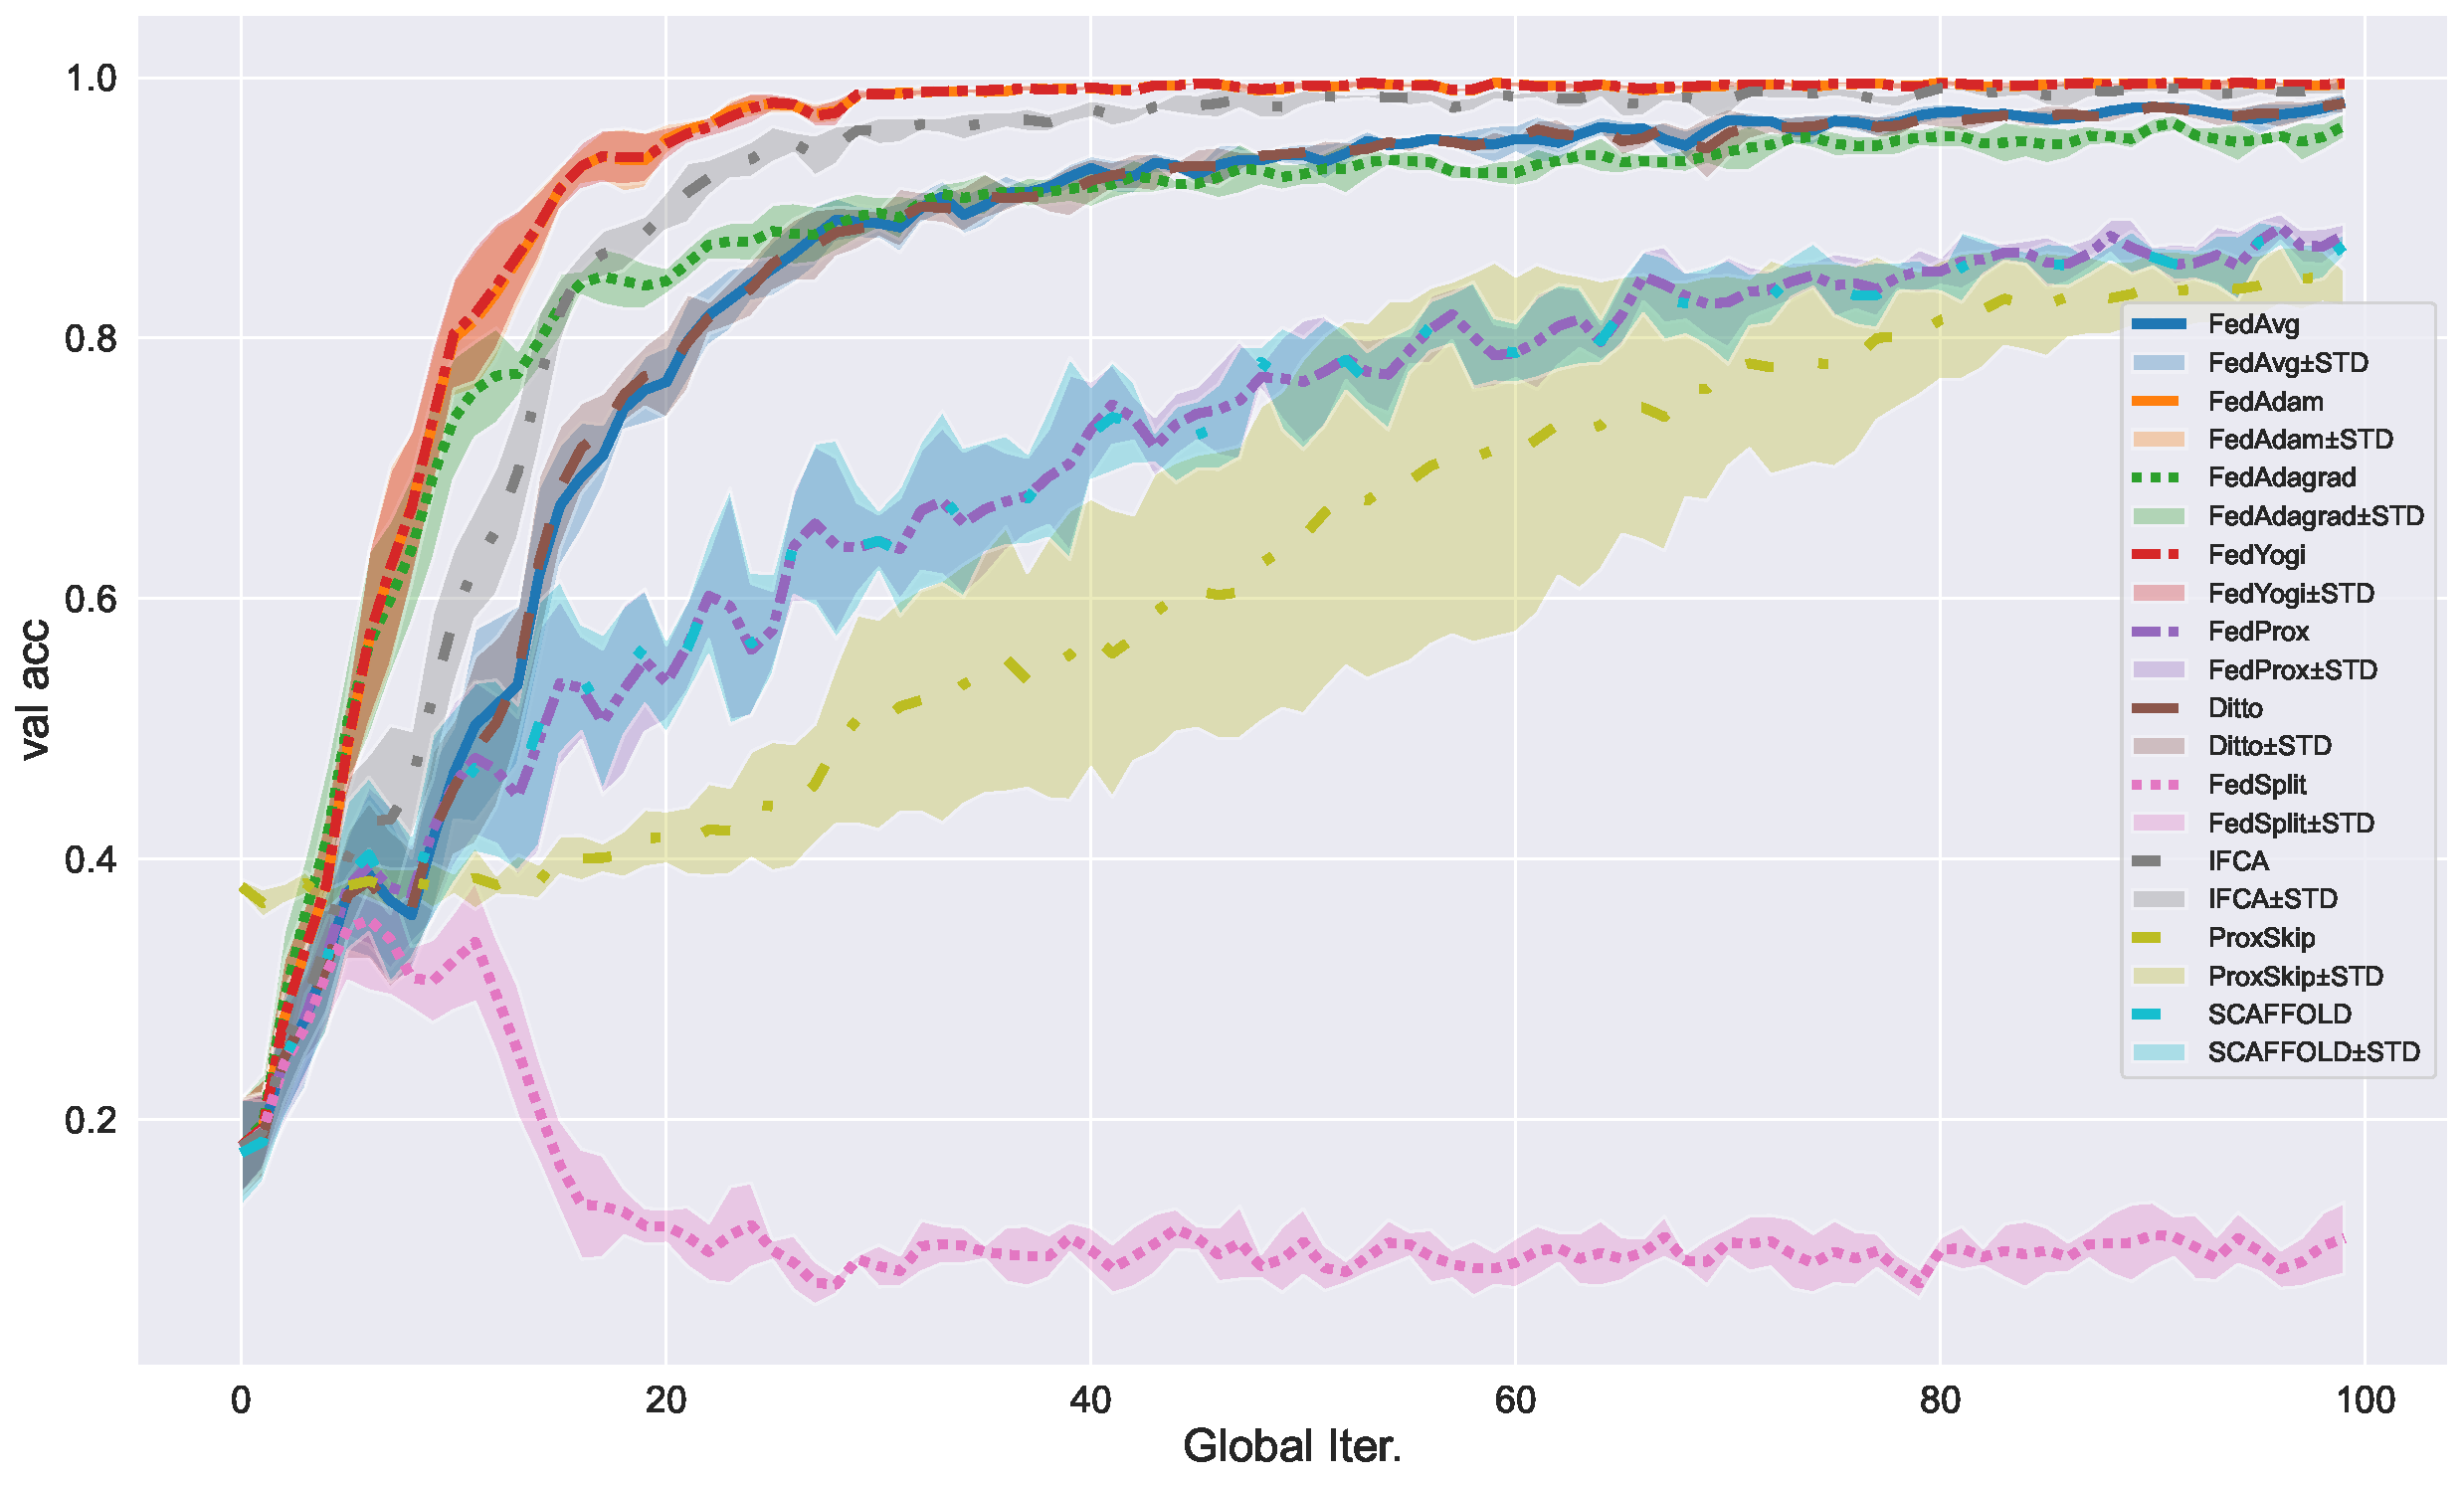
\includegraphics[width=0.9\textwidth]{figures/standard-test-ratio-30-val-acc.pdf}
    \caption{几种典型的联邦学习算法在子节点参与训练比例为$30\%$时,在测试集上的准确率曲线}
    \label{fig:standard-test-ratio-30-val-acc}
\end{figure}

\begin{figure}[ht]
    \centering
    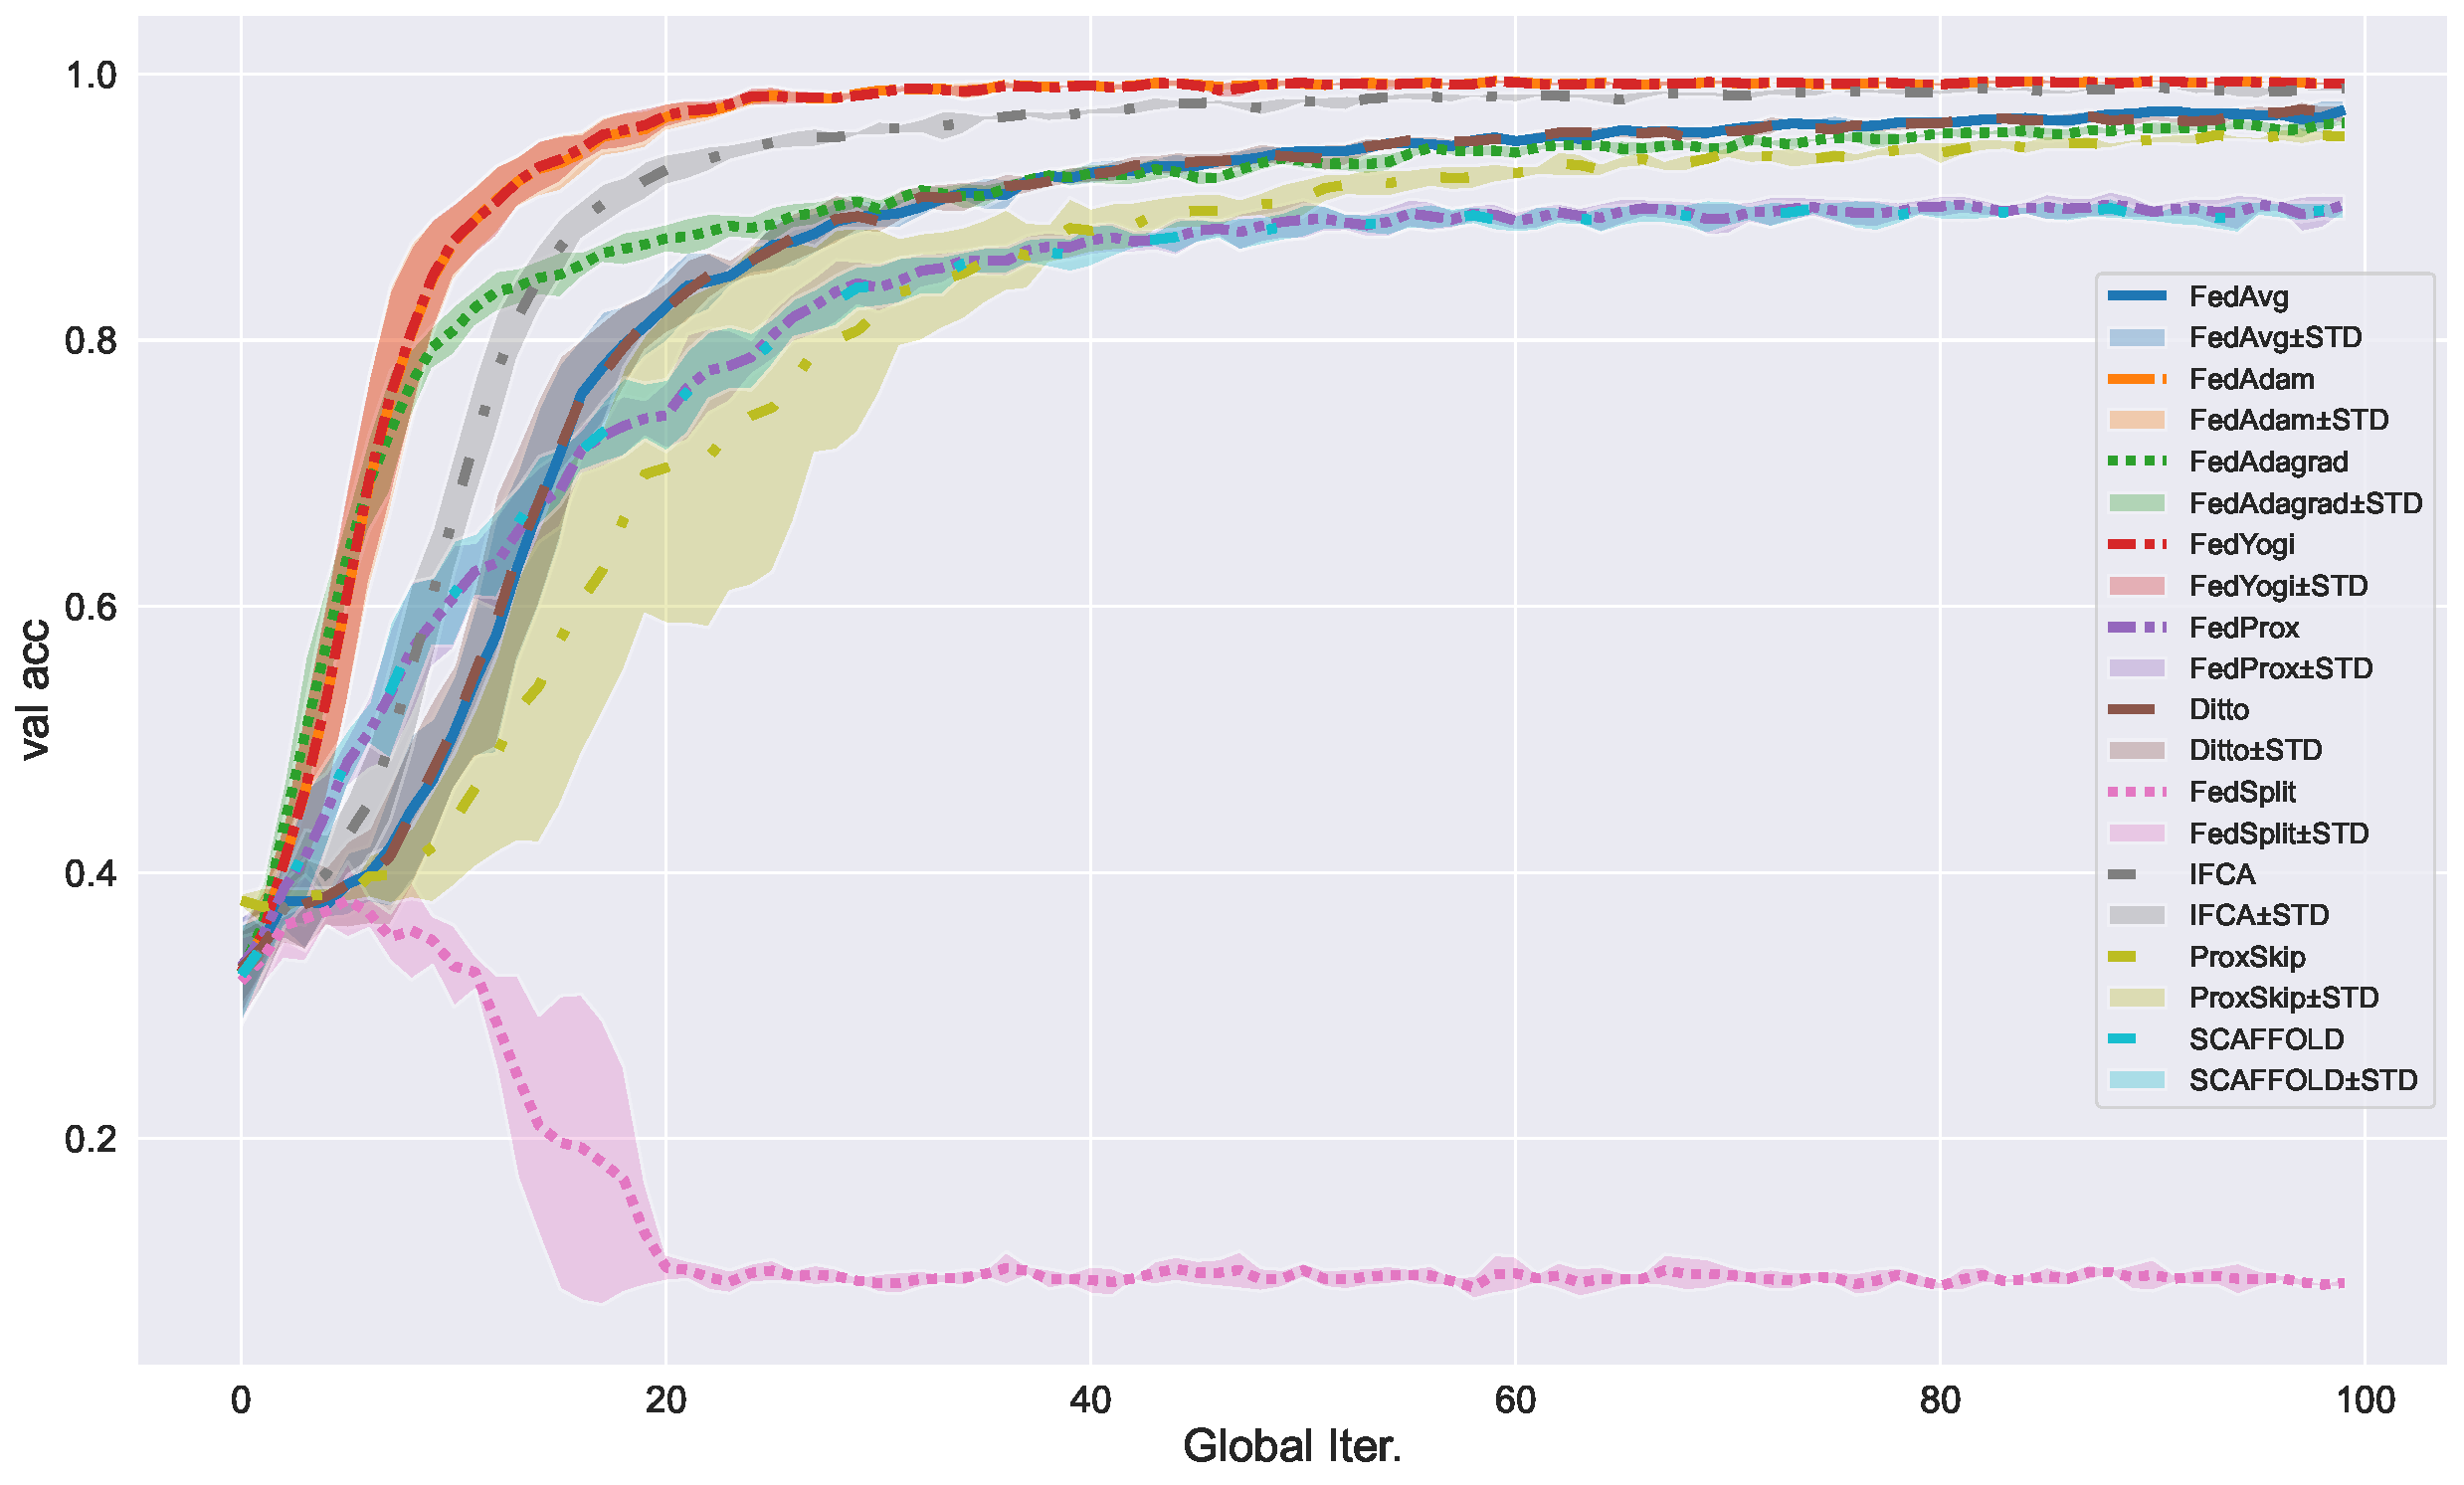
\includegraphics[width=0.9\textwidth]{figures/standard-test-ratio-70-val-acc.pdf}
    \caption{几种典型的联邦学习算法在子节点参与训练比例为$70\%$时,在测试集上的准确率曲线}
    \label{fig:standard-test-ratio-70-val-acc}
\end{figure}

\begin{figure}[ht]
    \centering
    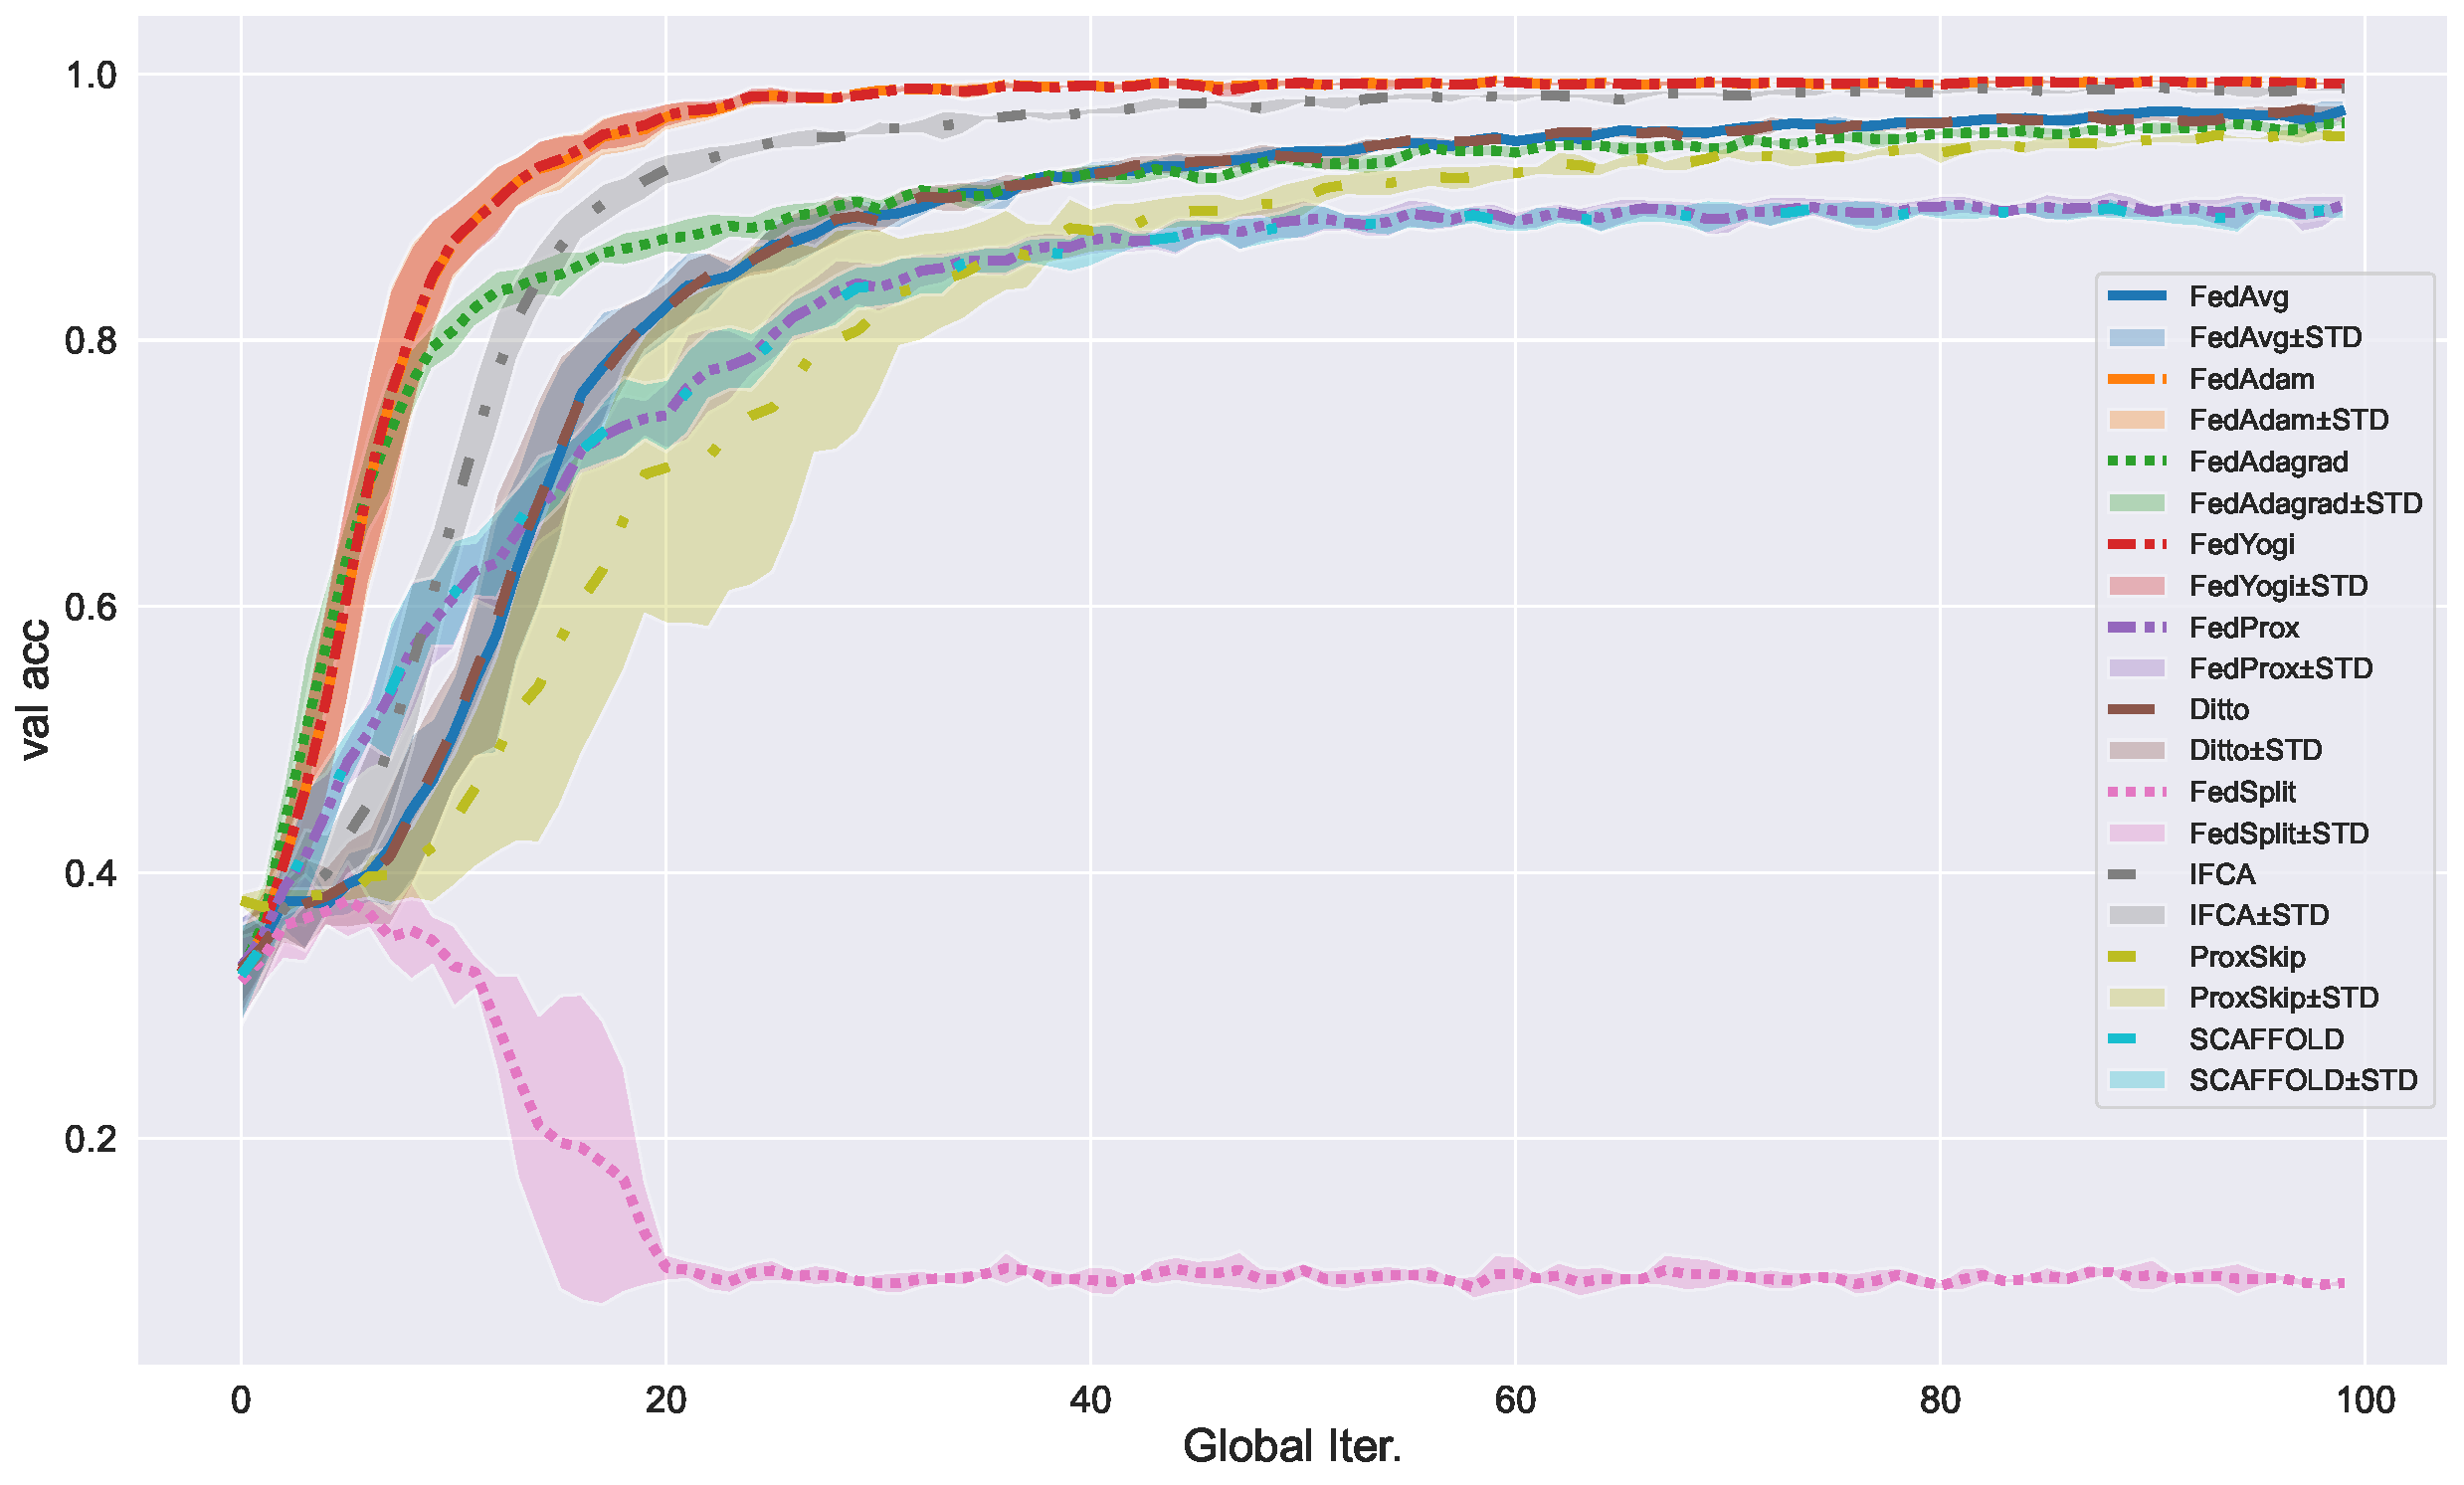
\includegraphics[width=0.9\textwidth]{figures/standard-test-ratio-70-val-acc.pdf}
    \caption{几种典型的联邦学习算法在子节点参与训练比例为$100\%$时,在测试集上的准确率曲线}
    \label{fig:standard-test-ratio-100-val-acc}
\end{figure}

图\ref{fig:standard-test-ratio-30-val-acc}, \ref{fig:standard-test-ratio-70-val-acc}, \ref{fig:standard-test-ratio-100-val-acc}~分别是这几种联邦学习优化算法在在子节点参与训练比例为$30\%,$ $70\%,$ 以及$100\%$时,在数据集\texttt{FedProxFEMNIST}的测试集上的准确率曲线。可以看到,随着每轮参与训练的子节点比例的提升,或者等价地,每一轮子节点掉队比例的降低,包括\texttt{FedProx}, \texttt{ProxSkip}在内的联邦学习优化算法的稳定性是逐渐提升的。而对于联邦分裂算法\texttt{FedSplit}来说,只有当子节点参与训练比例为$100\%$时才不发散,而且在这种情况下,其收敛速度也较慢。


\section{待写}
\addcontentsline{toe}{section}{{\currentchapter .2\ \ To write}\numberline\,}

% NOT finished

\begin{figure}[ht]
\centering
\begin{subfigure}{.5\textwidth}
  \centering
  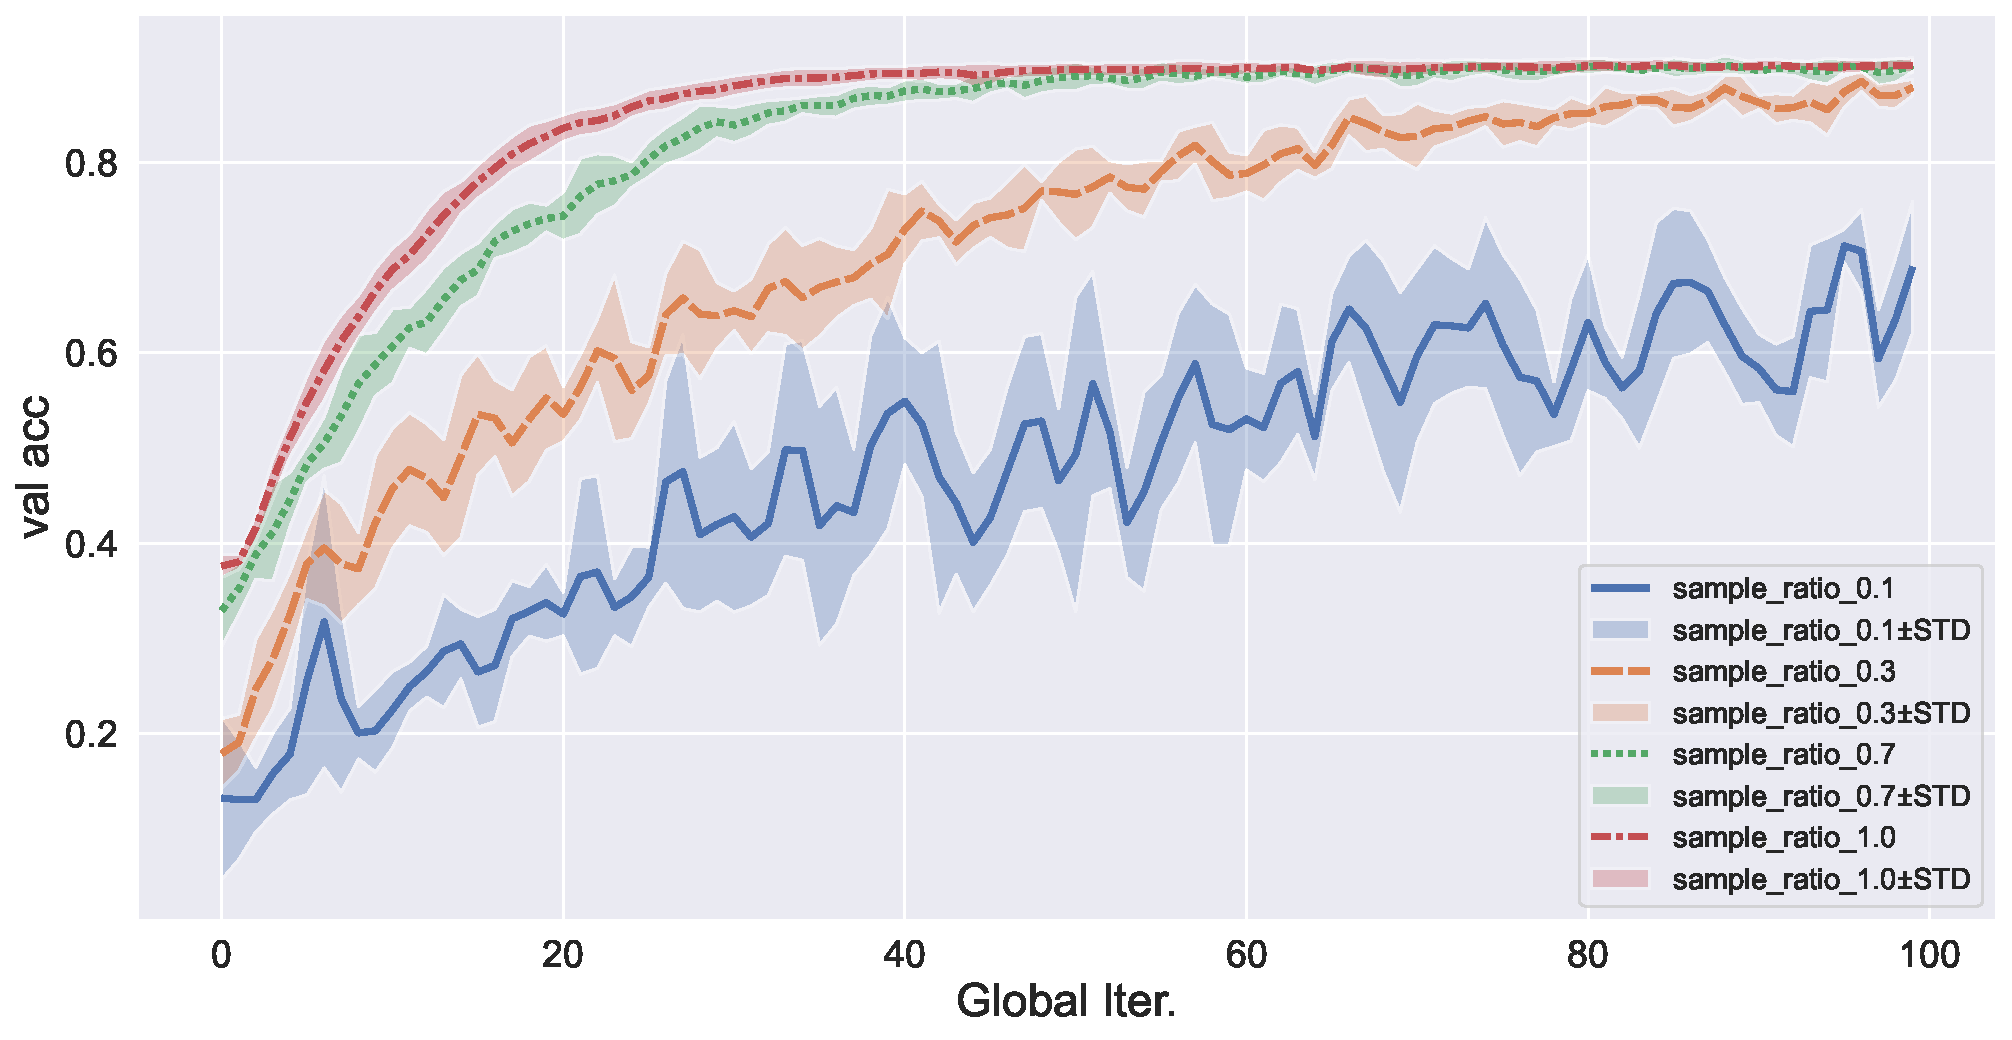
\includegraphics[width=.95\linewidth]{figures/fedprox-compare-sample-ratio-val-acc.pdf}
  \caption{xx}
  \label{fig:fedprox-compare-sample-ratio-val-acc}
\end{subfigure}%
\begin{subfigure}{.5\textwidth}
  \centering
  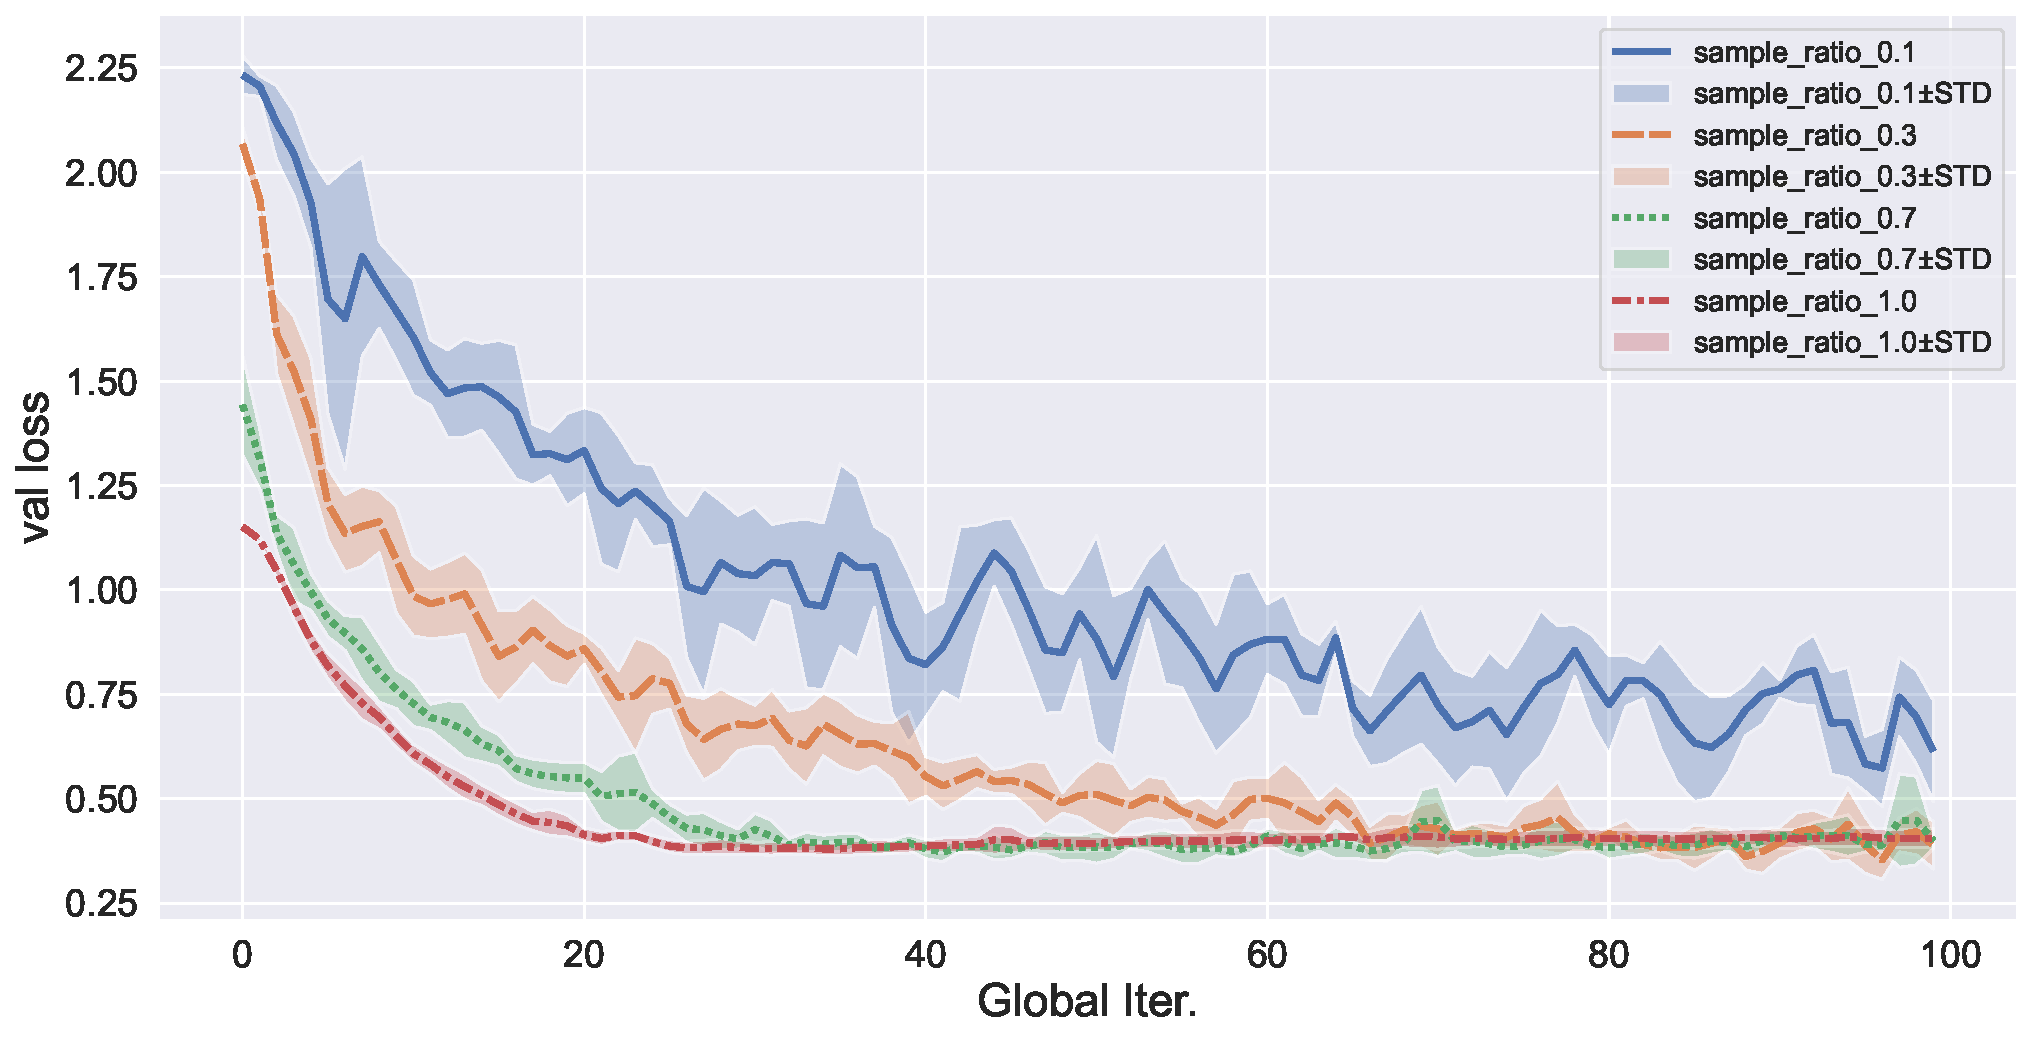
\includegraphics[width=.95\linewidth]{figures/fedprox-compare-sample-ratio-val-loss.pdf}
  \caption{xx}
  \label{fig:fedprox-compare-sample-ratio-val-loss}
\end{subfigure}
\begin{subfigure}{.5\textwidth}
  \centering
  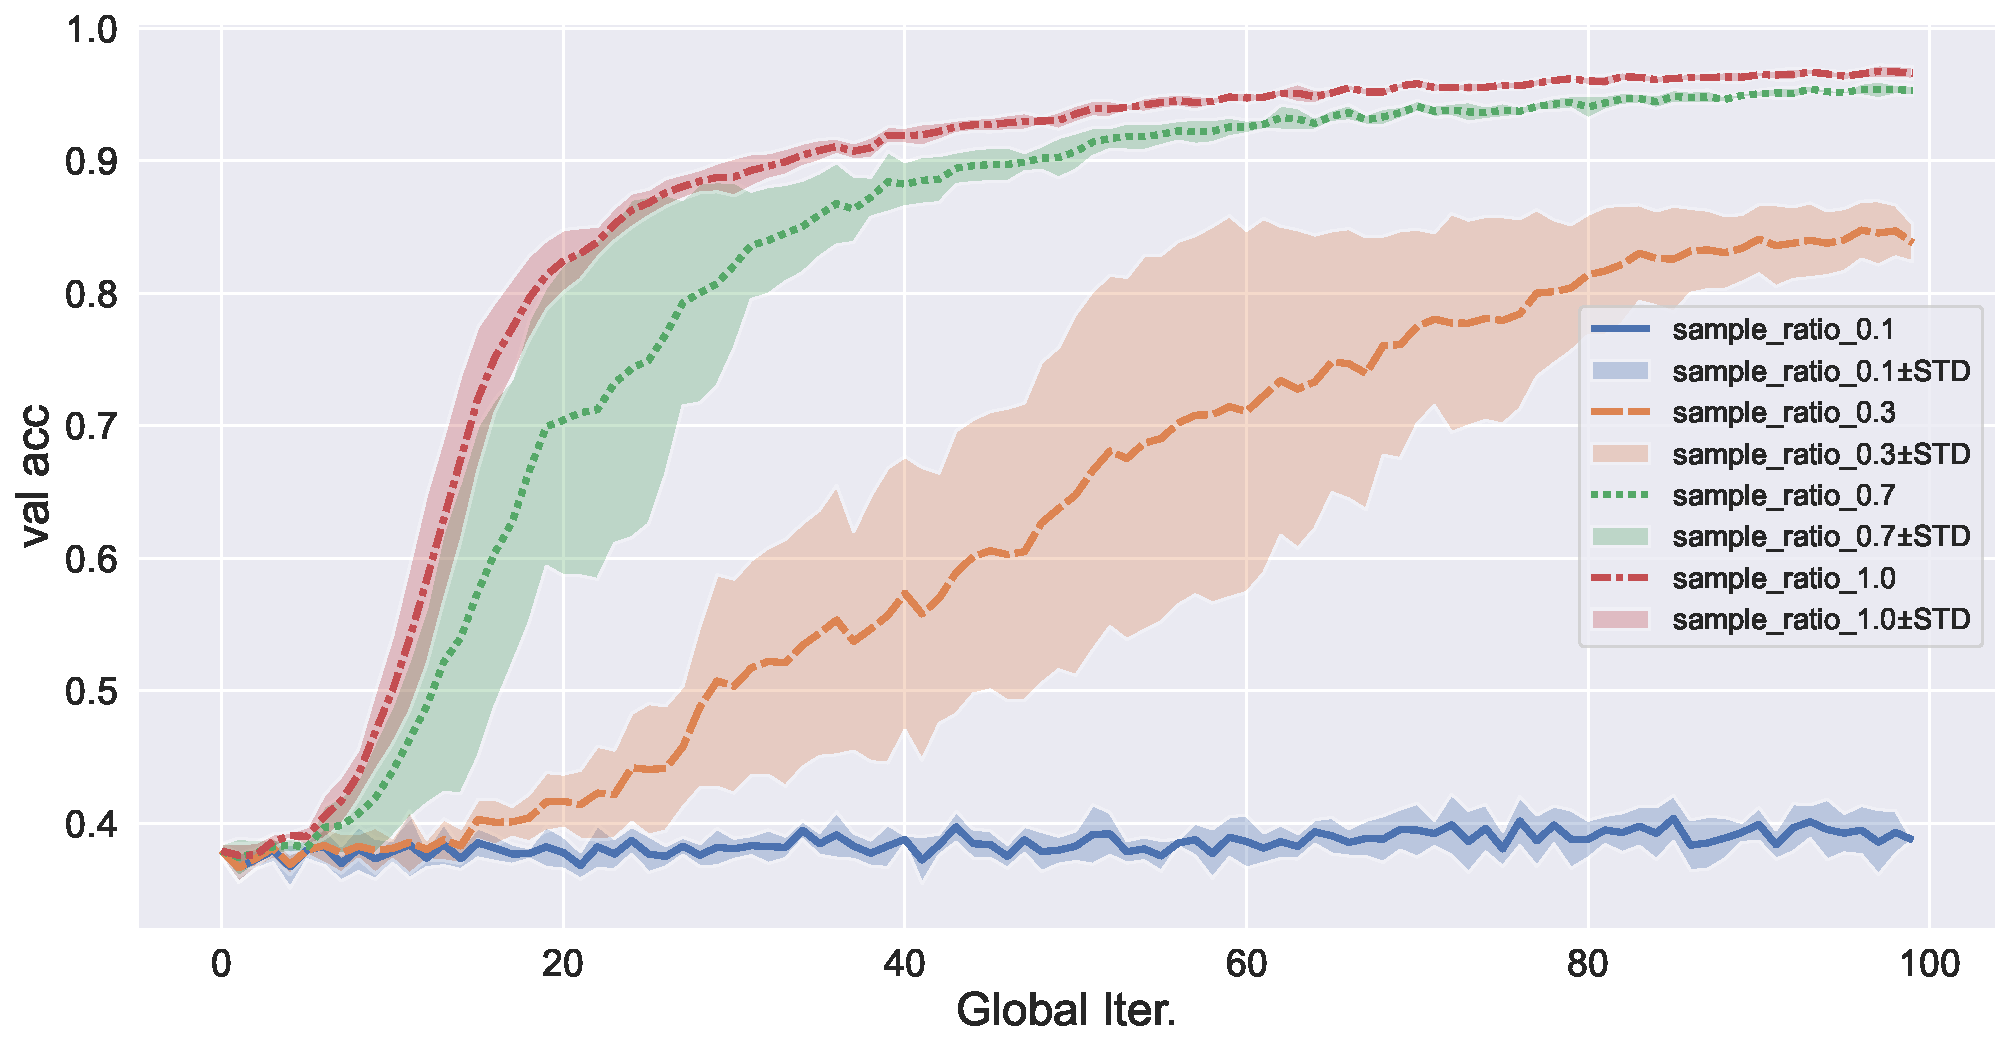
\includegraphics[width=.95\linewidth]{figures/proxskip-compare-sample-ratio-val-acc.pdf}
  \caption{xx}
  \label{fig:proxskip-compare-sample-ratio-val-acc}
\end{subfigure}%
\begin{subfigure}{.5\textwidth}
  \centering
  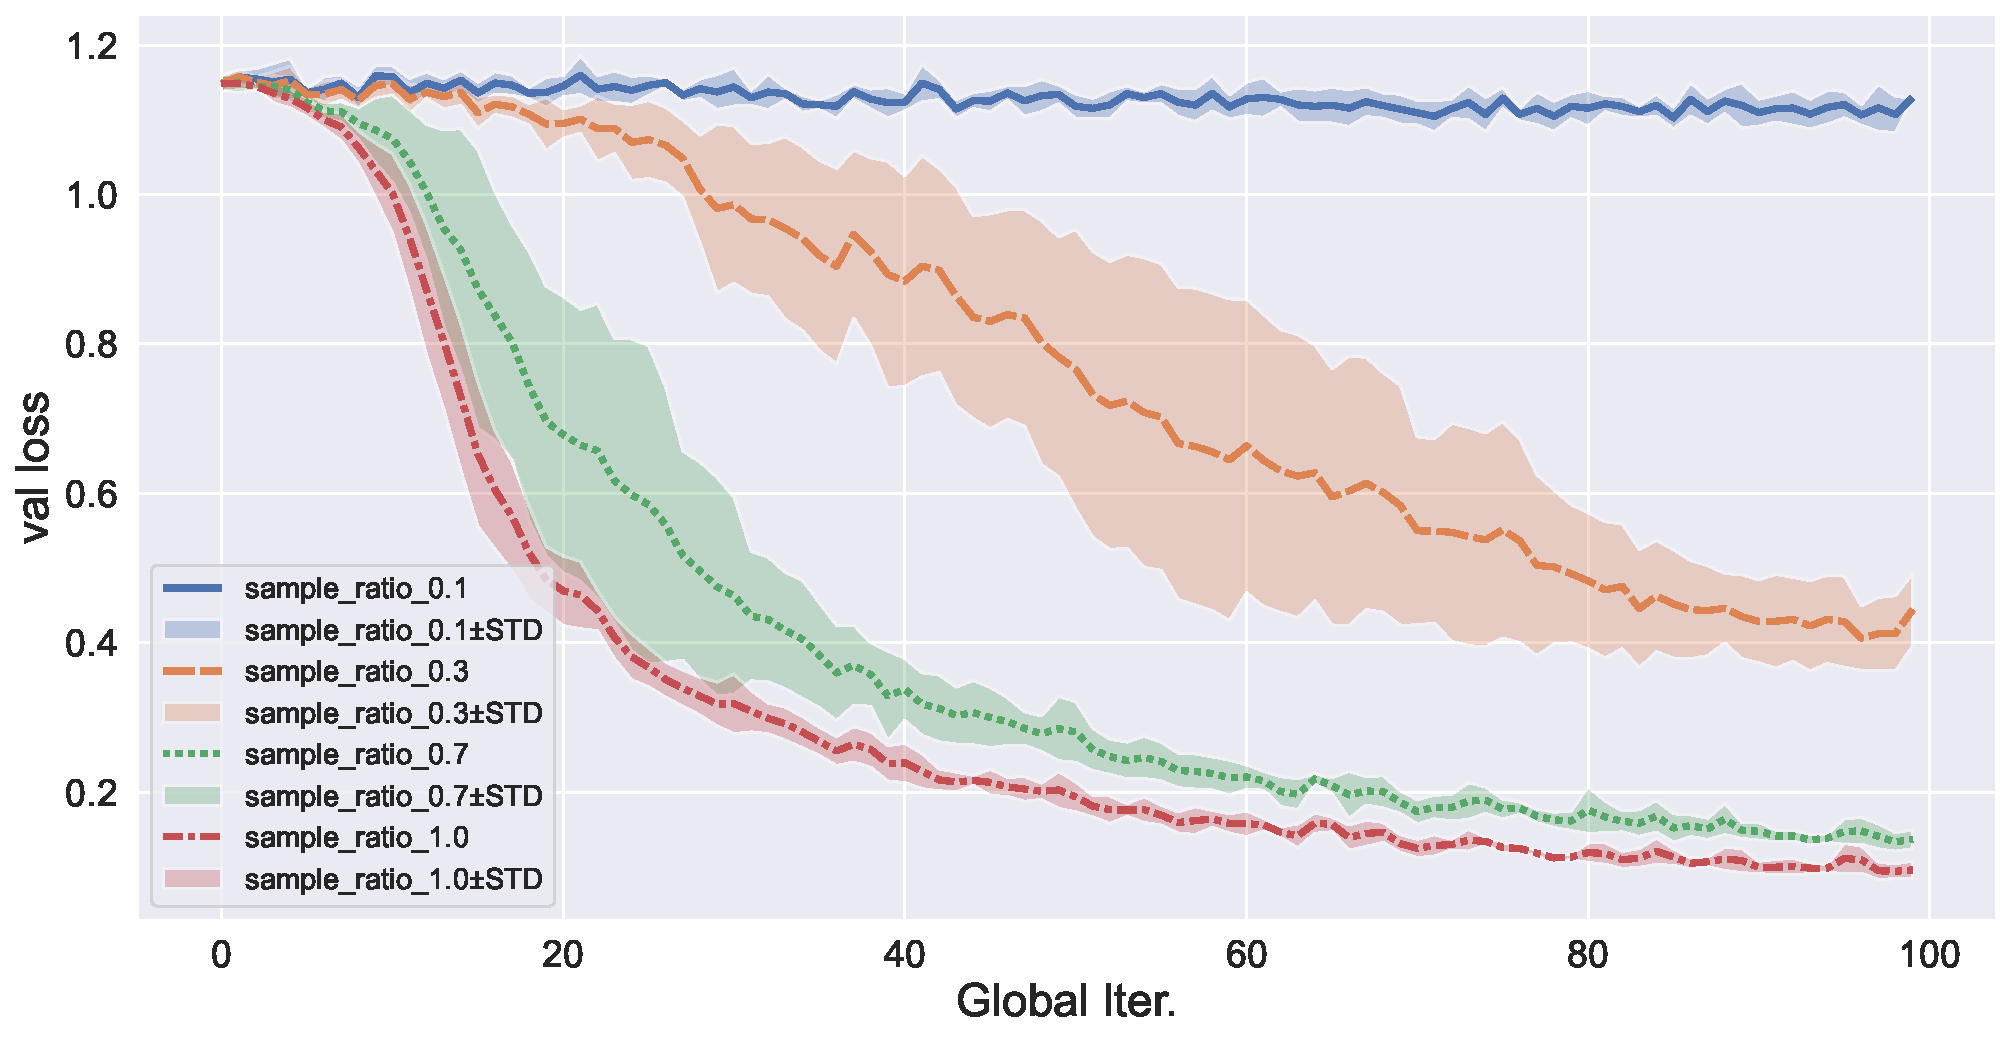
\includegraphics[width=.95\linewidth]{figures/proxskip-compare-sample-ratio-val-loss.pdf}
  \caption{xx}
  \label{fig:proxskip-compare-sample-ratio-val-loss}
\end{subfigure}
\begin{subfigure}{.5\textwidth}
  \centering
  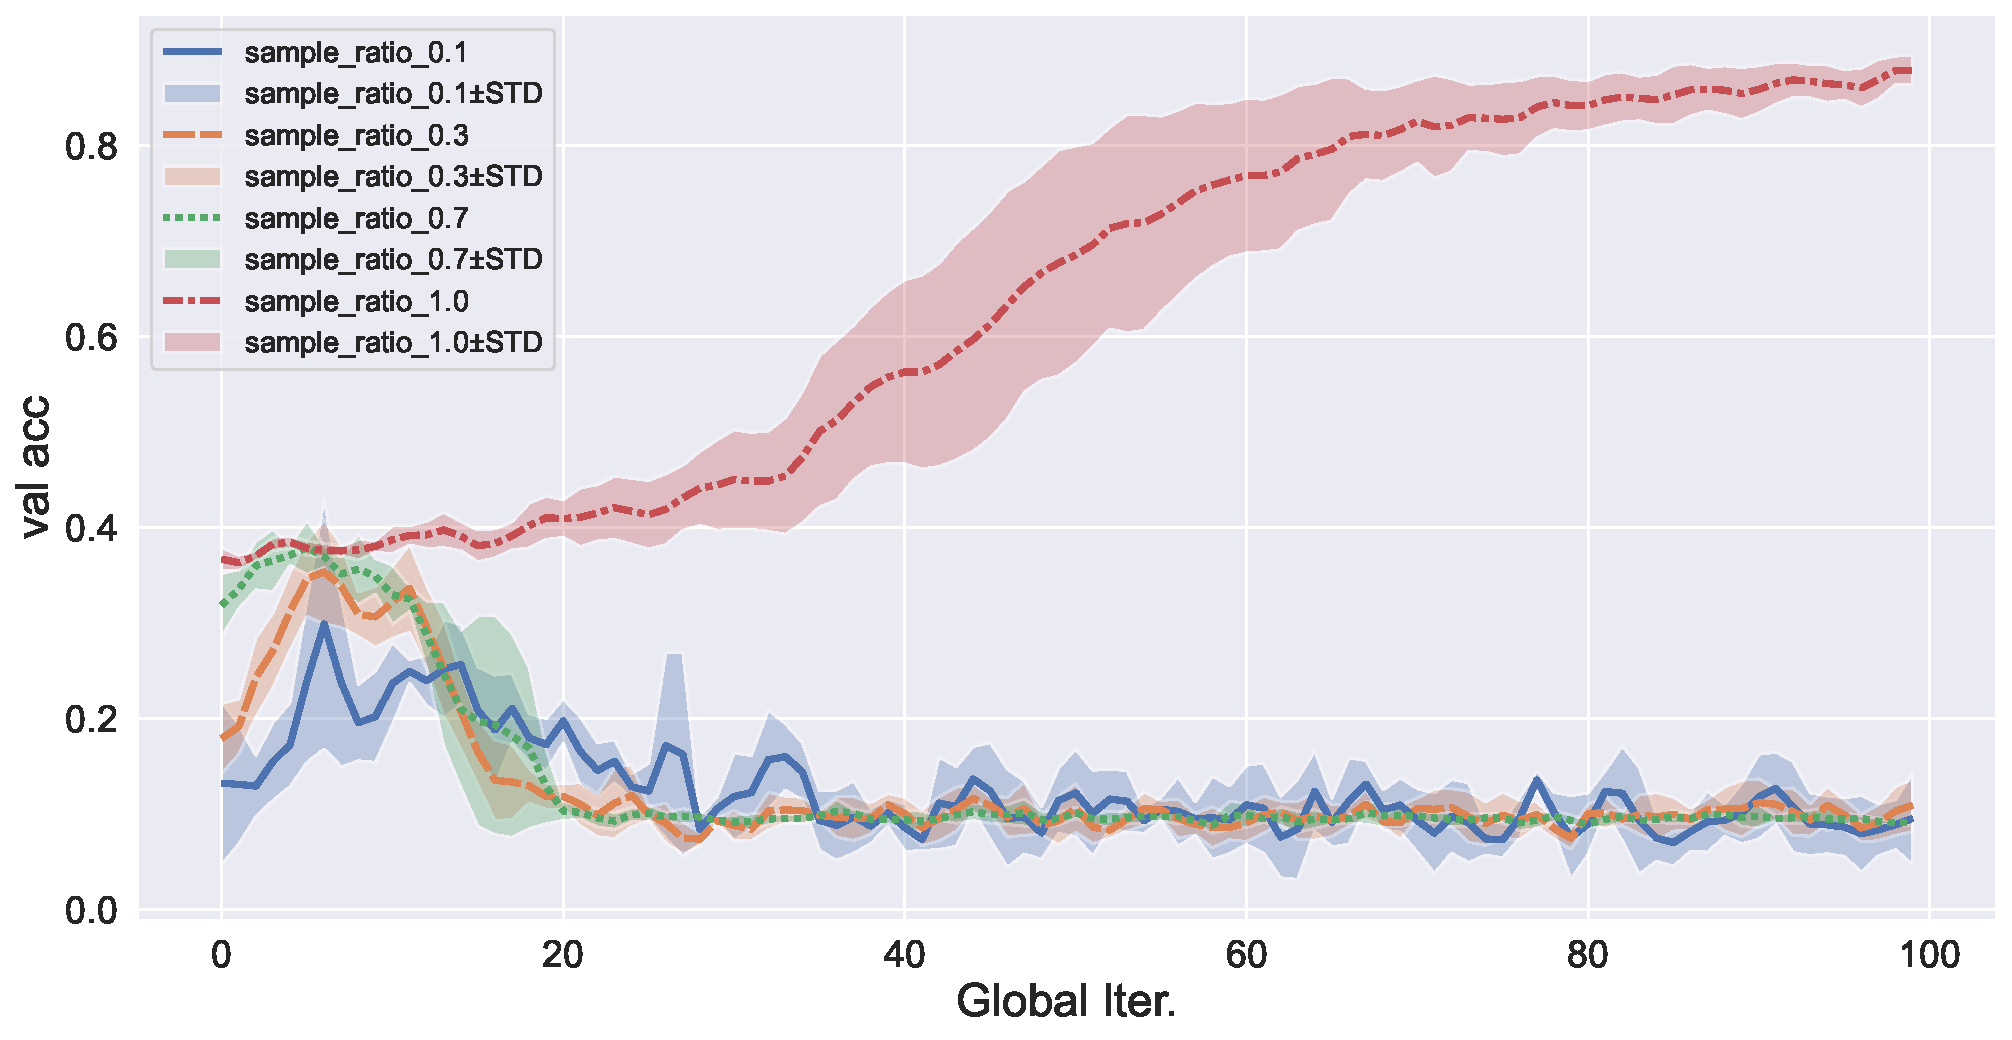
\includegraphics[width=.95\linewidth]{figures/fedsplit-compare-sample-ratio-val-acc.pdf}
  \caption{xx}
  \label{fig:fedsplit-compare-sample-ratio-val-acc}
\end{subfigure}%
\begin{subfigure}{.5\textwidth}
  \centering
  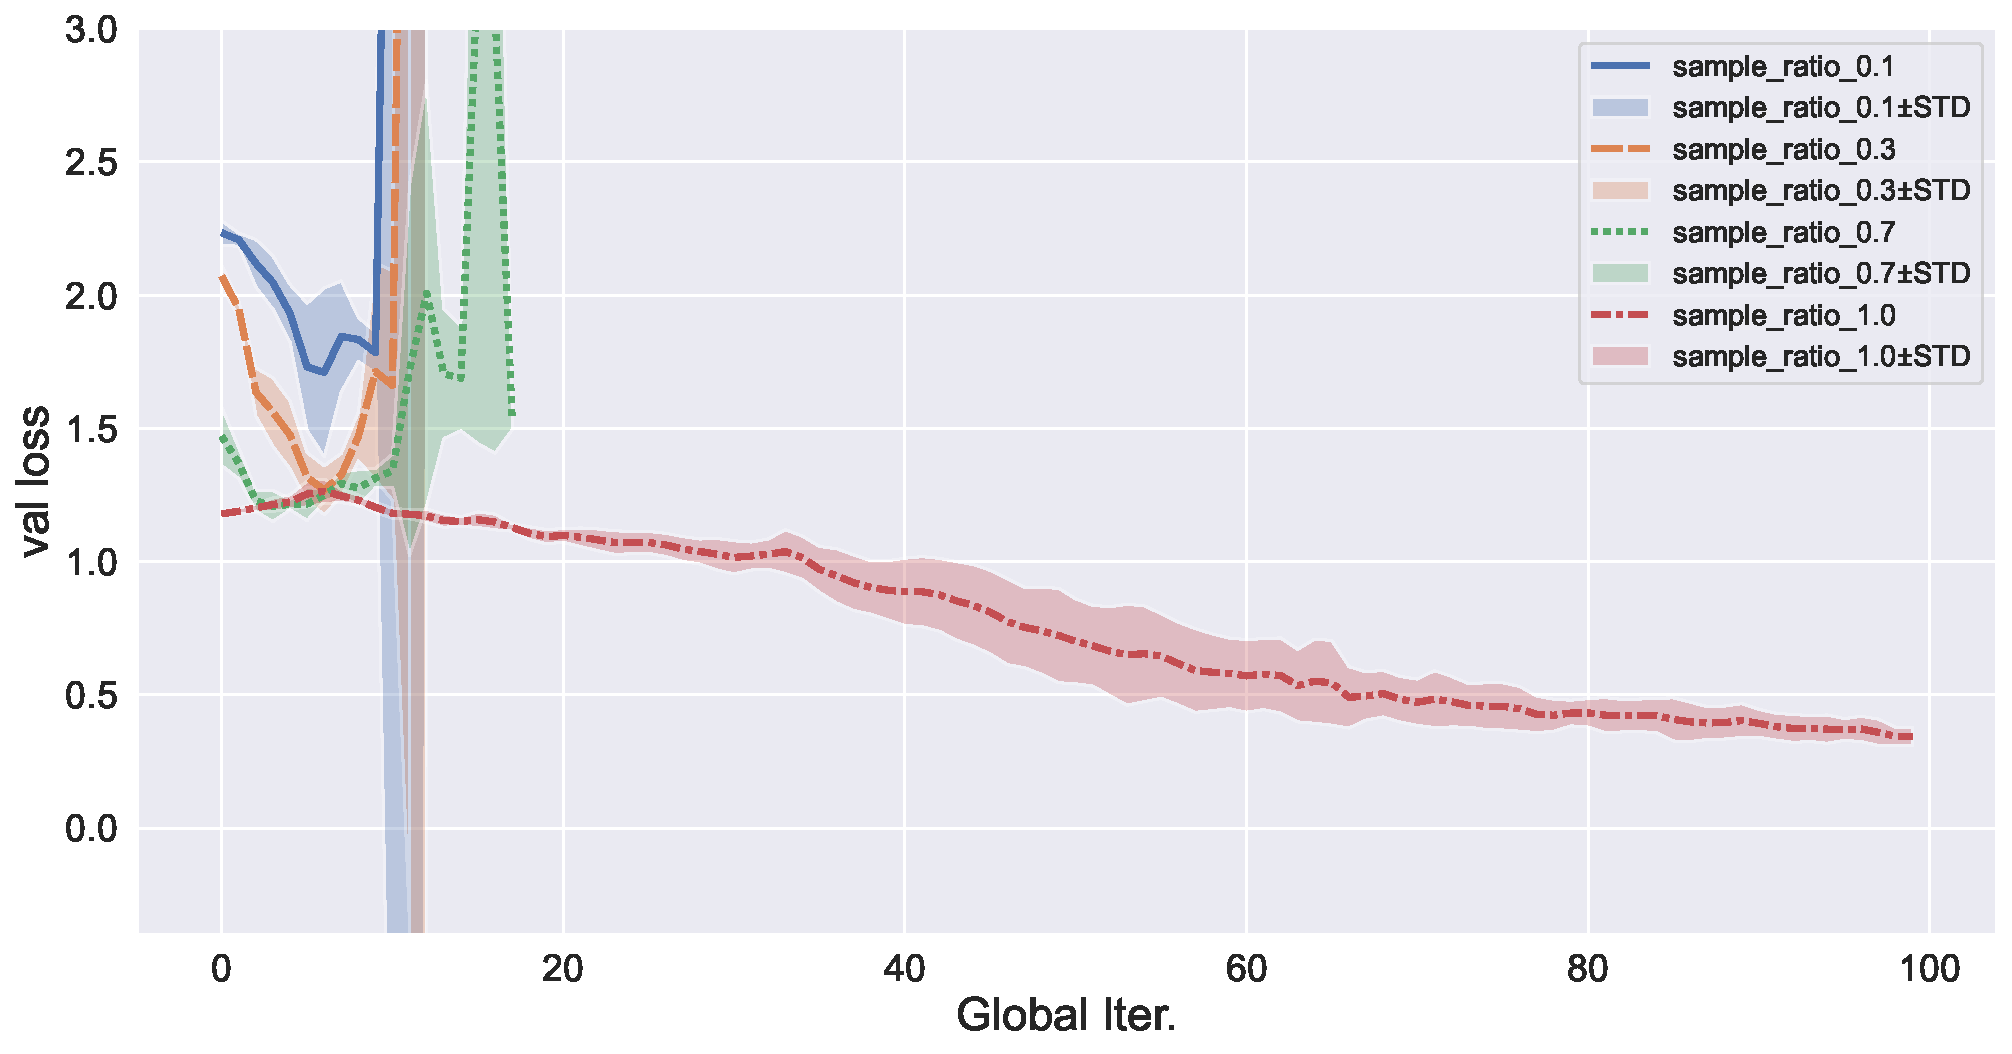
\includegraphics[width=.95\linewidth]{figures/fedsplit-compare-sample-ratio-val-loss.pdf}
  \caption{xx}
  \label{fig:fedsplit-compare-sample-ratio-val-loss}
\end{subfigure}
\begin{subfigure}{.5\textwidth}
  \centering
  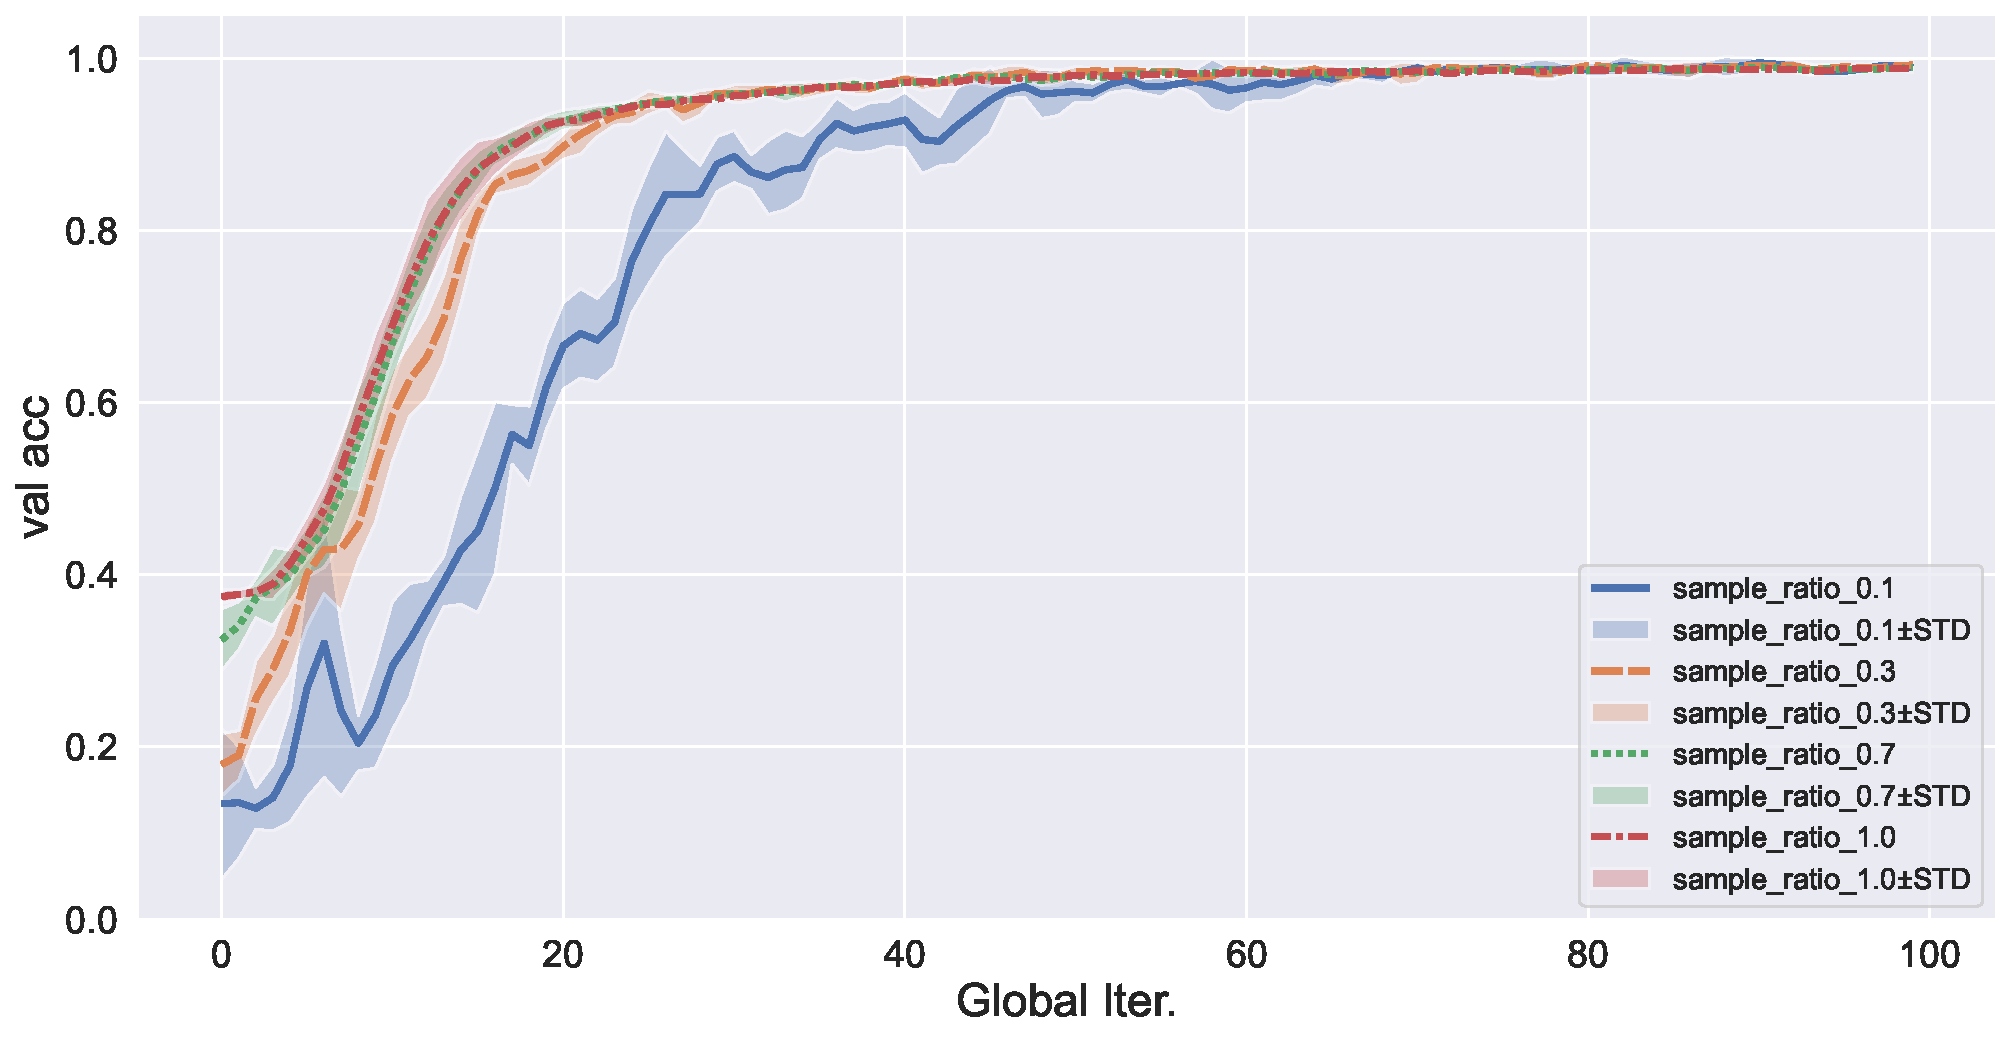
\includegraphics[width=.95\linewidth]{figures/ifca-compare-sample-ratio-val-acc.pdf}
  \caption{xx}
  \label{fig:ifca-compare-sample-ratio-val-acc}
\end{subfigure}%
\begin{subfigure}{.5\textwidth}
  \centering
  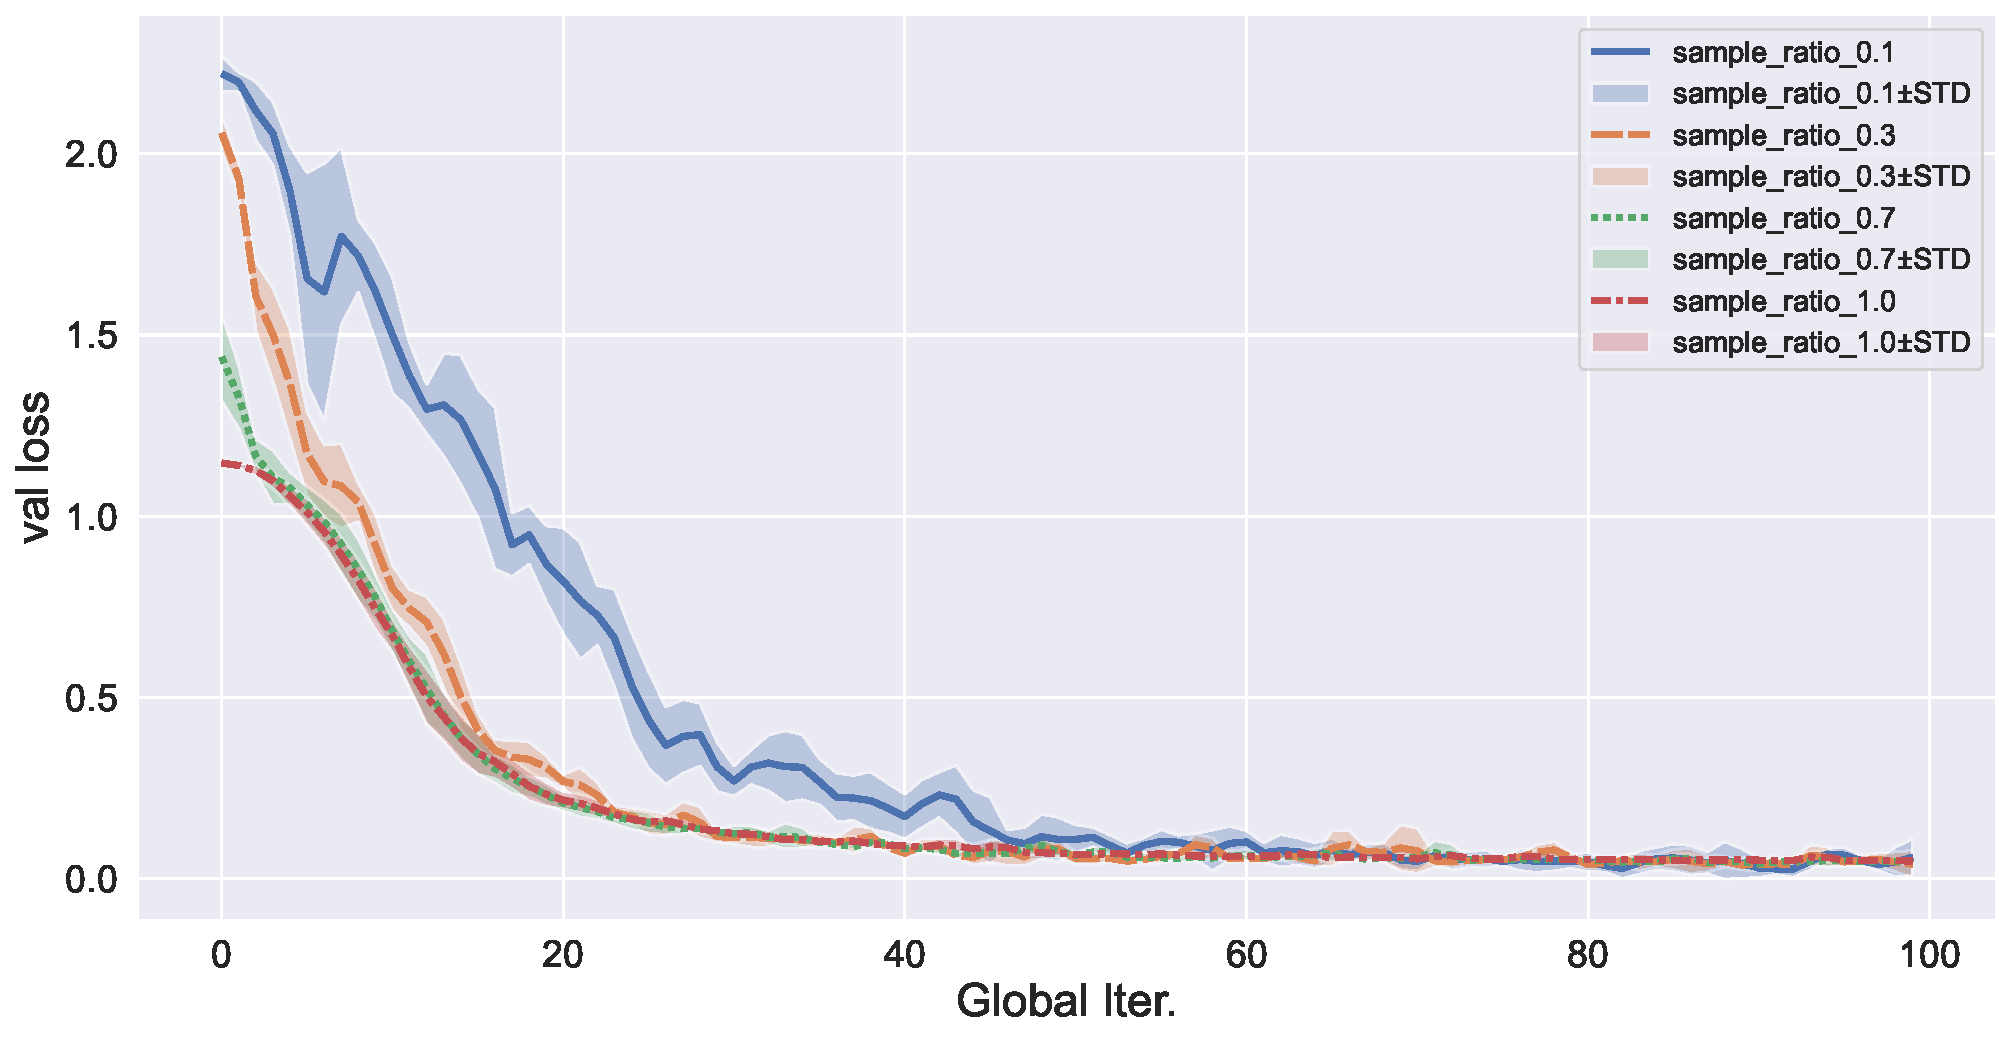
\includegraphics[width=.95\linewidth]{figures/ifca-compare-sample-ratio-val-loss.pdf}
  \caption{xx}
  \label{fig:ifca-compare-sample-ratio-val-loss}
\end{subfigure}
\caption{xx}
\label{fig:fedprox-compare-sample-ratio}
\end{figure}



待写。。。。

\section{待写}
\addcontentsline{toe}{section}{{\currentchapter .3\ \ To write}\numberline\,}

% NOT finished

\begin{figure}[ht]
\centering
\begin{subfigure}{.5\textwidth}
  \centering
  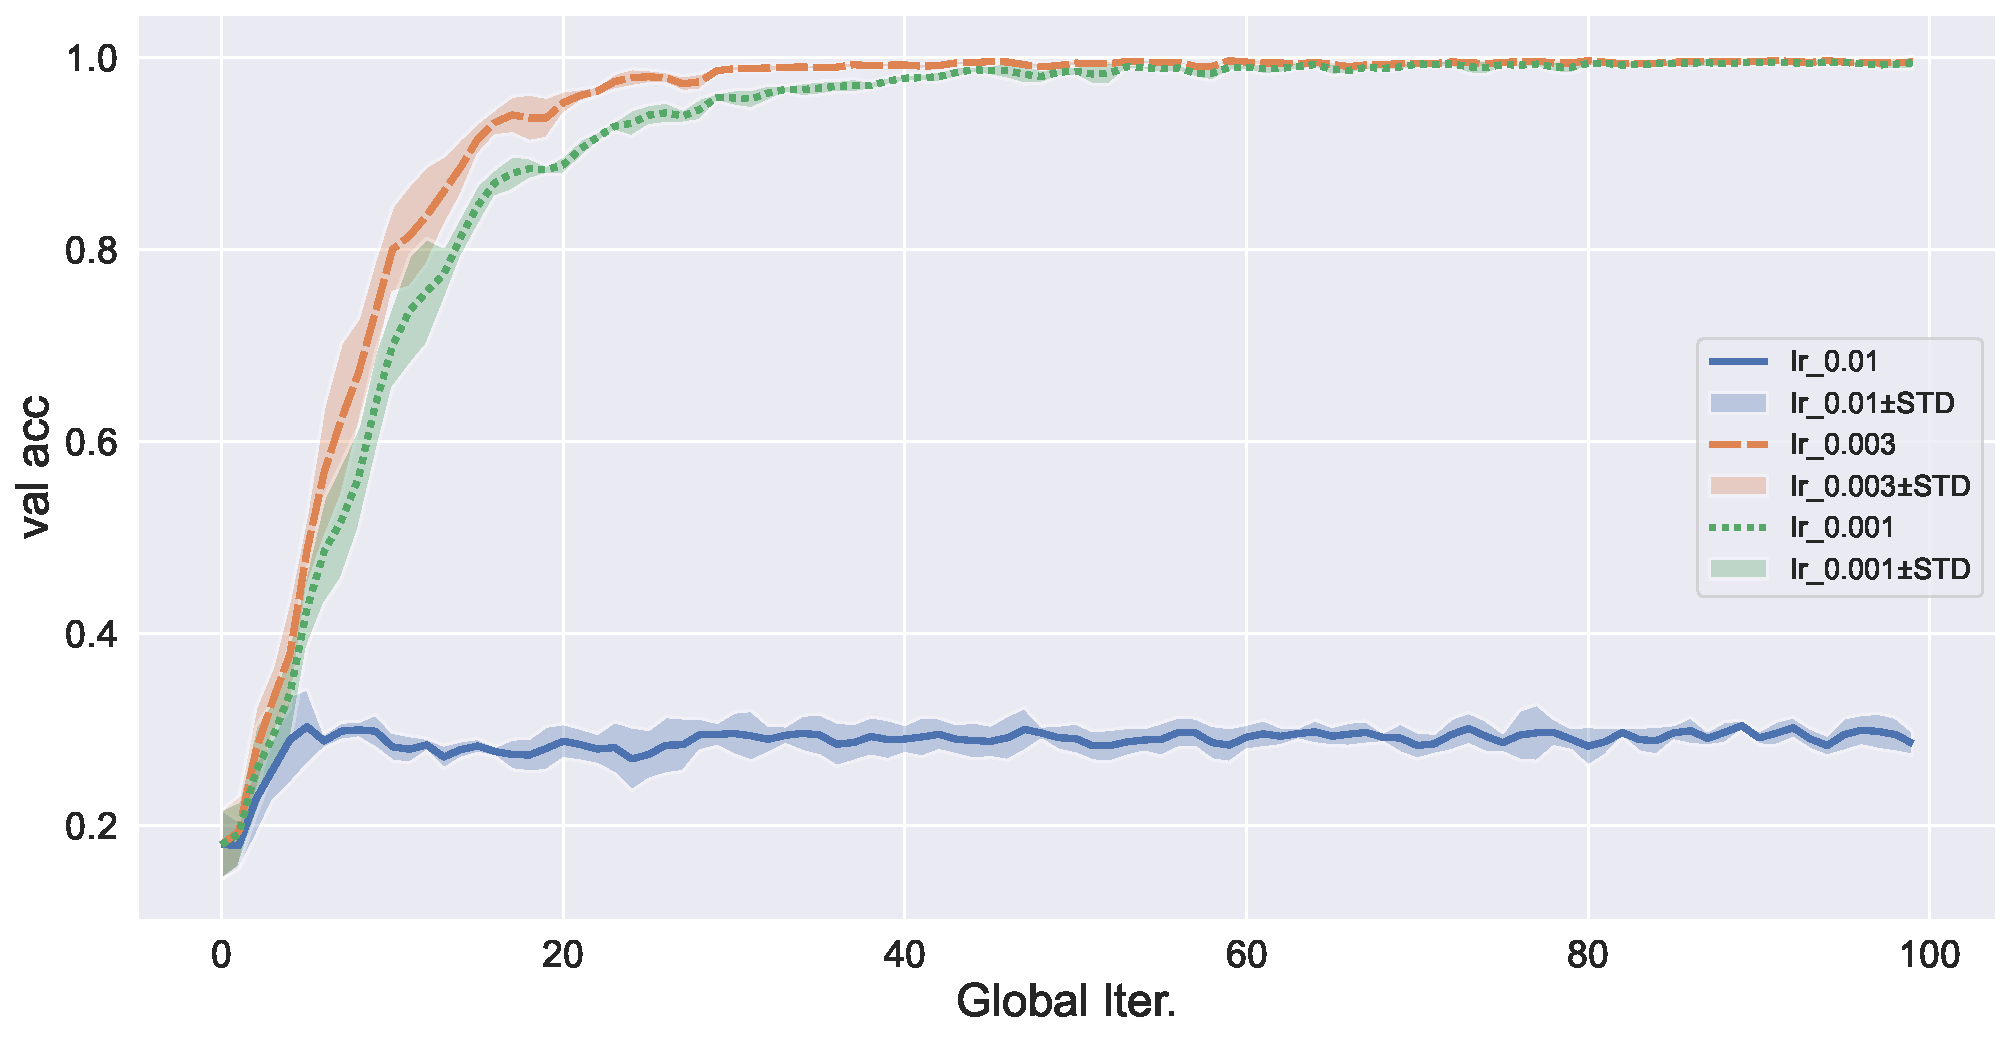
\includegraphics[width=.95\linewidth]{figures/adam-sample-30-compare-lr-val-acc.pdf}
  \caption{xx}
  \label{fig:adam-sample-30-compare-lr-val-acc}
\end{subfigure}%
\begin{subfigure}{.5\textwidth}
  \centering
  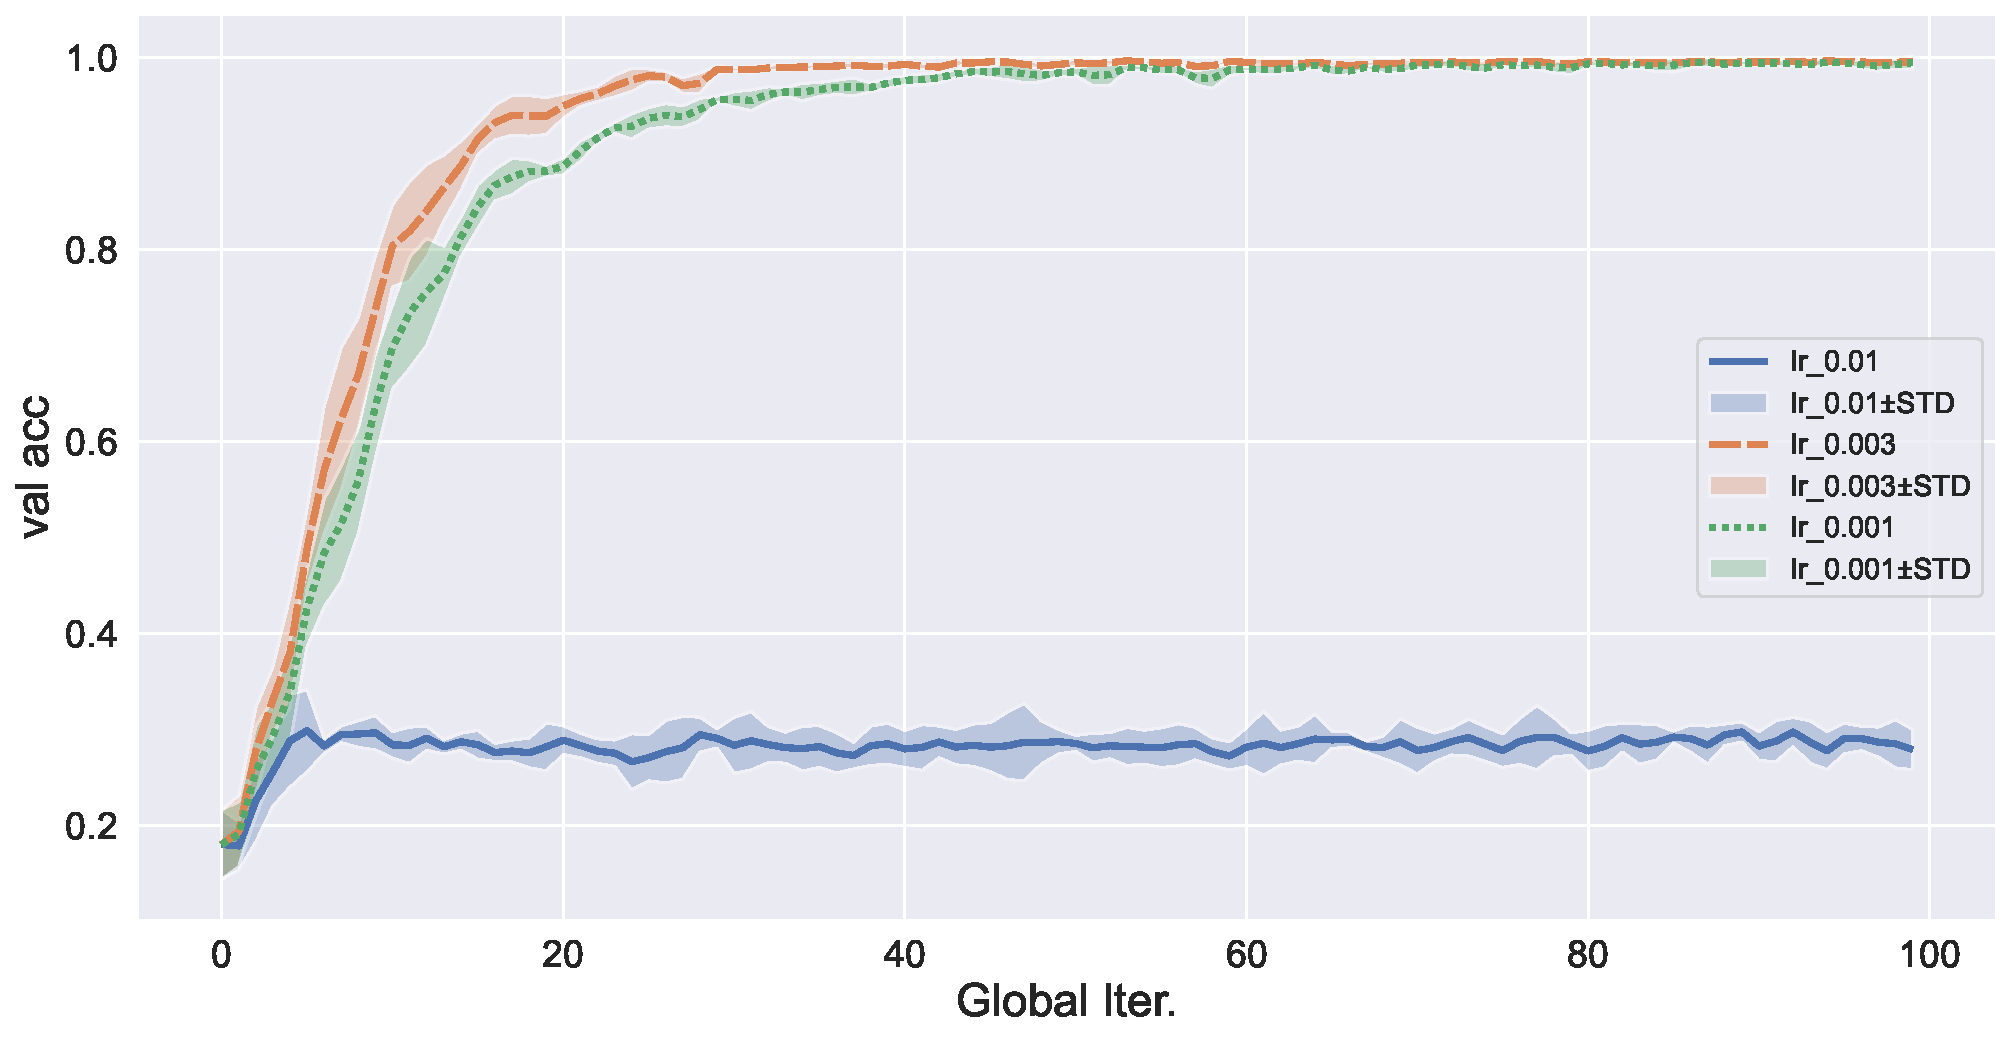
\includegraphics[width=.95\linewidth]{figures/yogi-sample-30-compare-lr-val-acc.pdf}
  \caption{xx}
  \label{fig:yogi-sample-30-compare-lr-val-acc}
\end{subfigure}
\begin{subfigure}{.6\textwidth}
  \centering
  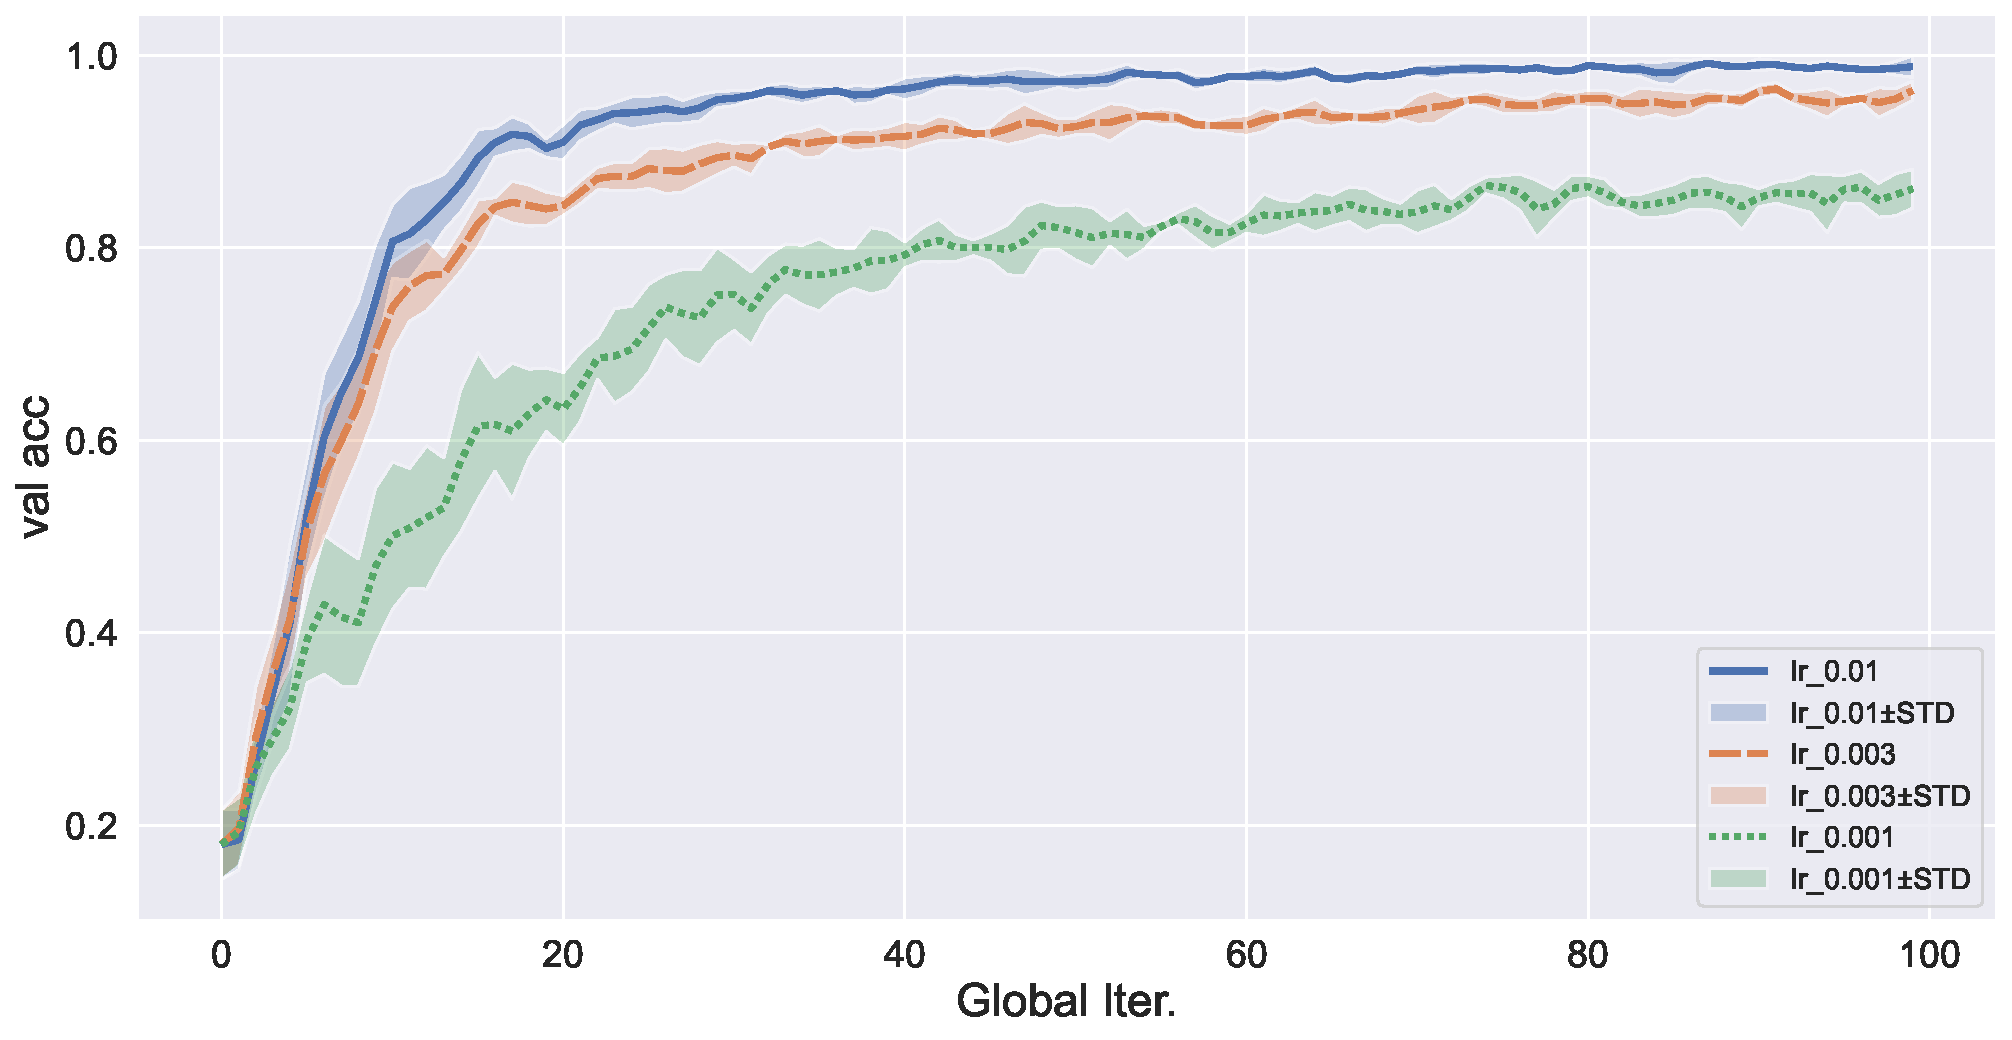
\includegraphics[width=.95\linewidth]{figures/adagrad-sample-30-compare-lr-val-acc.pdf}
  \caption{xx}
  \label{fig:adagrad-sample-30-compare-lr-val-acc}
\end{subfigure}
\caption{xx}
\label{fig:fedopt-sample-30-compare-lr-val-acc}
\end{figure}

待写。。。。
